 \documentclass[11pt]{article}

% ---------------------------------------------------------------
% Suitability of the actor model of concurrency for high-frequency trading
% arXiv preprint --- primary q-fin.TR (Trading & Market Microstructure);
% cross-list cs.DC
% ---------------------------------------------------------------

\usepackage[utf8]{inputenc}
\usepackage[T1]{fontenc}
\usepackage{lmodern}
\usepackage{amsmath,amssymb}
\usepackage{booktabs}
\usepackage{geometry}
\usepackage{hyperref}
\usepackage{xcolor}
\usepackage{enumitem}
\usepackage[ruled,vlined,linesnumbered]{algorithm2e}
\usepackage{microtype}
\usepackage{caption}
% Captions get their own font: smaller than body, bold "Table/Figure N." label.
\captionsetup{font=small, labelfont=bf, labelsep=period}
\usepackage{tikz}
\usetikzlibrary{arrows.meta,positioning,fit,backgrounds,calc}
\usepackage{pgfplots}
\pgfplotsset{compat=1.18}
\usepackage{placeins}
\usepackage{graphicx}
\usepackage{draftwatermark}
\SetWatermarkText{DRAFT}
\SetWatermarkScale{1.1}
\SetWatermarkColor[gray]{0.92}
% Give small tables/figures room to sit near their text rather than flushing to the end.
\renewcommand{\topfraction}{0.9}
\renewcommand{\bottomfraction}{0.8}
\renewcommand{\textfraction}{0.07}
\renewcommand{\floatpagefraction}{0.75}
\setcounter{topnumber}{3}
\setcounter{bottomnumber}{2}
\setcounter{totalnumber}{5}
\geometry{margin=1in}
\hypersetup{colorlinks=true, linkcolor=blue!50!black, citecolor=blue!50!black,
            urlcolor=blue!50!black}

\newcommand{\fs}{\texttt{fast\_send}}
\newcommand{\snd}{\texttt{send}}

\title{\textbf{Suitability of the Actor Model of Concurrency for\\
High-Frequency Trading}\\
\large The \texttt{fast\_send} Mechanism and a Tick-to-Book Latency Study}

\author{%
  Vincent Maciejewski\\
  \small M2 Technologies\\
  \small \texttt{mayeski@gmail.com}
}

\date{September 2026}

\begin{document}
\maketitle

\begin{abstract}
The many benefits of the actor model --- per-actor state isolation, freedom
from data races and deadlocks, and sequential single-message reasoning --- have
been recognized for decades, yet the model has long been dismissed as unsuitable
for high-frequency trading (HFT). The reasoning was that actors imply many
threads, many mailbox queues, and a message --- with its heap allocation, queue
operations, scheduler dispatch, and context switch --- for every interaction:
overhead incompatible with a microsecond latency budget. This paper argues that
the dismissal is wrong for co-located actors, and supports the argument not only
analytically but with a deployed, measured implementation --- \emph{kaspar-hft},
an open-source C++20 framework that extends the actor model into a form suitable
for HFT and is its reference implementation. The extensions are four: \fs{}, a
synchronous delivery
mechanism in which the sending thread runs the receiver's handler inline and
takes the reply as a value; actor \emph{groups}, which co-schedule a set of actors
on one thread behind a single shared mailbox; selectable mailbox queue
implementations matched per actor to its write pattern; and a memory pool that
removes per-message allocation and its tail.

The central mechanism is \fs{}, whose defining property is \emph{receiver
transparency}: the handler is written identically for synchronous and
asynchronous delivery and has no programmatic means to determine which was used,
which thread executes it, or whether the sender is blocked. Synchronous delivery
across a chain of grouped actors runs entirely on the first actor's thread,
reducing scheduler context switches from $O(N)$ on the asynchronous path to
$O(1)$; a thread-local call-chain test detects cyclic synchronous invocation
before any lock is taken; and five delivery operations expose the
latency/robustness spectrum behind one transparent interface. Microbenchmarks put
the synchronous round trip at tens of nanoseconds --- roughly two orders of
magnitude below the ungrouped asynchronous path --- and the pool cuts the
allocator tail by two orders of magnitude.

We then measure the framework in a real HFT setting: socket-to-book
(``tick-to-book'') latency on a live CME market-data feed for ES, NQ, and ZN
futures. The latency decomposes into a $\sim\!7~\mu$s decode-and-book floor plus a
per-message serialization slope, and the framework's own per-message contribution
is under $1\%$ of the floor. The tail is set not by the actor machinery or the
mailbox queue --- which is convex, as queueing theory predicts, but fires on
$0.08\%$ of messages --- but by the arrival process, which is non-Poisson and
self-exciting (Hawkes-like, branching ratio $0.85$--$0.97$). The latency the
concurrency model adds is thus minor next to the irreducible latencies a real HFT
data path already endures. Finally, the shared-queue group yields a
production/simulation duality: the same actor code runs unchanged in live trading
and in deterministic backtest. A saturated-throughput and contention evaluation
is left to future work.
\end{abstract}

\vspace{0.5em}
\noindent\textbf{Keywords:} actor model, message passing, concurrency,
synchronous delivery, deadlock detection, receiver transparency, low-latency
systems.

% ---------------------------------------------------------------
\section{Introduction}
% ---------------------------------------------------------------

In the actor model \cite{hewitt1973,agha1986}, a program is a collection of
isolated actors, each with private state, a message handler, and a mailbox.
Actors communicate only by asynchronous message passing: a sender places a
message on the receiver's mailbox and proceeds without waiting, and the receiver
dequeues and processes messages one at a time on its own thread. This discipline
is what gives the model its guarantees --- isolation, sequential per-actor
processing, and location transparency --- and it is essential when actors are
distributed across machines.

When the communicating actors reside in the same process on the same machine,
however, the asynchronous path carries overhead that the isolation guarantee
does not require. A single request-and-reply between two co-located actors
incurs, on conventional implementations:

\begin{itemize}[leftmargin=1.4em]
  \item \textbf{Heap allocation.} Because the message must outlive the sender's
  current continuation and persist until processed at an indeterminate later
  time, it must be heap-allocated, with the associated allocation cost,
  fragmentation, and garbage-collection pressure.
  \item \textbf{Queue operations.} Each message is enqueued by the sender and
  dequeued by the receiver, each requiring synchronization on the mailbox.
  \item \textbf{Scheduling and context switches.} The receiver must be scheduled
  onto a thread to run, incurring a context switch; a context switch typically
  costs on the order of $10^3$--$10^4$ processor cycles and pollutes cache and translation lookaside buffer (TLB) state.
  \item \textbf{Round-trip latency.} A reply repeats the entire path in reverse,
  so a request-and-reply crosses the mailbox twice and the scheduler twice.
\end{itemize}

For a same-process pair, all of this is avoidable in principle: the sender's own
thread could run the receiver's handler directly and take the reply as a return
value. The difficulty is doing so without breaking the abstraction the actor
model exists to provide. A direct handler invocation --- calling the receiver's
handler as an ordinary method --- discards the receiver's exclusive-execution
guarantee and exposes the receiver as a passive object. The design problem is to obtain the
performance of a direct, same-thread call while preserving, from the receiver's
point of view, the semantics of message passing.

This paper describes \fs{}, a synchronous delivery mechanism that resolves that
tension. The sending thread acquires exclusive access to the receiving actor and
executes the receiver's handler directly, on the sender's thread, returning the
reply as a value. The receiver's handler is identical for synchronous and
asynchronous delivery and cannot determine which was used --- the property we
call \emph{receiver transparency}. Because synchronous invocations can form
cycles, and a cycle deadlocks a non-reentrant lock or overflows the stack under
a reentrant one, the mechanism carries a lightweight cyclic-invocation detector
that fires before any lock is taken. \fs{} is implemented in \emph{kaspar-hft}, an
open-source C++20 actor framework for high-frequency
trading;\footnote{\url{https://github.com/vincent212/kaspar-hft}} all code and
measurements in this paper are drawn from that repository.

\paragraph{Contributions.}
\begin{enumerate}[leftmargin=1.6em]
  \item A synchronous, same-thread actor-delivery mechanism (\fs{}) that
  eliminates the heap allocation, queue operations, scheduling, and context
  switches of the asynchronous path for co-located actors, and returns the reply
  as a value (Section~\ref{sec:mech}).
  \item A precise statement and enforcement of \emph{receiver transparency}: the
  handler executes identical code in both modes and cannot determine the
  delivery mode, the executing thread, or whether the sender is blocked
  (Section~\ref{sec:transparency}).
  \item A thread-local call-chain membership test that detects cyclic
  synchronous invocation before lock acquisition, together with a refined
  (actor, message-class) variant that admits callback patterns while still
  catching unbounded recursion (Section~\ref{sec:cycle}).
  \item A family of five delivery operations spanning asynchronous through
  spin-wait synchronous to best-effort-with-async-fallback, unified behind one
  transparent handler interface (Section~\ref{sec:family}).
  \item An analytical account of the per-message work eliminated, together with
  microbenchmarks of the C++ implementation that measure each eliminated
  operation and the pool's tail benefit; a saturated-throughput evaluation is
  left to future work (Section~\ref{sec:perf}).
\end{enumerate}

% ---------------------------------------------------------------
\section{Origins and history of the actor model}
\label{sec:history}
% ---------------------------------------------------------------

\paragraph{Invention (1973).} The actor model was introduced by Carl Hewitt,
Peter Bishop, and Richard Steiger in ``A Universal Modular ACTOR Formalism for
Artificial Intelligence,'' presented at the Third International Joint Conference
on Artificial Intelligence (IJCAI) at Stanford in August 1973
\cite{hewitt1973}. Its origins were in artificial-intelligence research at MIT:
the formalism grew out of Hewitt's earlier work on the PLANNER language and was
proposed as a single, uniform notion --- the \emph{actor}, an entity that
communicates only by sending messages to other actors --- rich enough to serve
as a foundation for AI programming. Hewitt drew on the object and
message-sending ideas of Simula~67 and Smalltalk, on Lisp, and on capability
systems, Petri nets, and packet-switched networks; in later retrospectives he
described the model as inspired by the laws of physics rather than by any
prior computational abstraction \cite{hewitt2010}.

\paragraph{Formal foundations (1975--1986).} The 1973 paper was informal, and a
decade of work followed to give the model a rigorous semantics. Irene Greif's
1975 MIT doctoral thesis supplied the first operational semantics for actor
computations \cite{greif1975}; Hewitt and Baker stated ``laws'' characterizing
the partial ordering of events in a distributed actor computation
\cite{hewittbaker1977}; and William Clinger's 1981 thesis gave a denotational
semantics based on power domains, addressing the unbounded nondeterminism that
distinguishes actors from other concurrency formalisms \cite{clinger1981}. The
foundation most cited today is Gul Agha's doctoral work, published as
\emph{Actors: A Model of Concurrent Computation in Distributed Systems}
\cite{agha1986}, which recast the model with a transition-system operational
semantics built on the primitives \emph{create}, \emph{send}, and \emph{become},
and moved the emphasis from artificial intelligence to a general theory of
open, concurrent, distributed computation.

\paragraph{From theory to practice.} The most influential early
\emph{deployed} system with actor-like structure --- isolated processes with
private state that communicate only by asynchronous message passing --- was
Erlang, developed at Ericsson from 1986 by Joe Armstrong, Robert Virding, and
Mike Williams for fault-tolerant telephony \cite{armstrong1996}. The historical
relationship to Hewitt's model is often overstated: Erlang's designers have said
they were unaware of the actor model while building the language, and Armstrong
later characterized Erlang's concurrency as closer in spirit to communicating
sequential processes than to the actor model \cite{armstrong2007}. Erlang is
therefore best understood as a parallel, largely independent arrival at similar
principles rather than a direct descendant, even though it is now routinely
described as an actor language. Hewitt himself continued to revise the model's
definition well after 1973, emphasizing unbounded nondeterminism, locality, and
guaranteed delivery in a much later retrospective \cite{hewitt2010}. The
subsequent two decades produced a broad ecosystem of practical actor
runtimes --- on the JVM, the .NET platform, C++, Rust, Swift, and elsewhere ---
which we survey next.

% ---------------------------------------------------------------
\section{A survey of actor-model implementations}
\label{sec:survey}
% ---------------------------------------------------------------

This section surveys the major actor runtimes along the three axes most relevant
to \fs{}: how actors are mapped to operating-system threads, whether and how a
synchronous or request--reply path is offered, and what is known of their
performance. The consistent findings across the ecosystem --- that actors are
multiplexed M:N over a small worker pool, and that no mainstream system runs the
\emph{receiver's} handler on the \emph{sender's} thread --- are what locate the
contribution of \fs{}. Table~\ref{tab:survey} summarizes the comparison; the
per-system detail and performance figures follow. The later related-work
discussion (Section~\ref{sec:related}) revisits the systems closest to \fs{} to
sharpen the distinction; here the account is descriptive.

\begin{table}[t]
\centering
\caption{Actor-to-thread mapping and synchronous messaging across
implementations. The final column --- whether the sender's thread ever executes
the receiver's message handler --- is negative for every surveyed system and
positive only for \fs{}.}
\label{tab:survey}
\footnotesize
\setlength{\tabcolsep}{4pt}
\begin{tabular}{p{2.2cm} p{1.8cm} p{3.1cm} p{3.0cm} c}
\toprule
System & Runtime & Actor $\to$ thread mapping & Synchronous / request--reply & Sender runs handler? \\
\midrule
Erlang/OTP, Elixir & BEAM VM & M:N green processes; one scheduler thread per core; per-scheduler run queues, work stealing & \texttt{gen\_server:call} blocks caller, returns a value; handler runs in the server process & No \\
Akka & JVM & thread-pool dispatchers over a fork--join pool; actors not 1:1 with threads & \texttt{ask} (\texttt{?}) returns a \texttt{Future}; \texttt{tell} (\texttt{!}) is fire-and-forget & No \\
Akka.NET, Orleans & .NET & thread-pool / turn-based scheduling; grains single-threaded per activation & grain methods return \texttt{Task<T>}; always asynchronous & No \\
CAF & C++ & cooperative work-stealing scheduler over $P{=}\#\text{cores}$ workers; \texttt{detached} actors get a thread & \texttt{request} returns a response handle; \texttt{.then} continuation, non-blocking & No \\
SObjectizer & C++ & agents bound to dispatchers supplying worker threads/pools & async by default; \texttt{so5extra} \texttt{request\_reply} blocks; runs on provider's dispatcher & No \\
Actix & Rust / Tokio & actors are tasks on Arbiter event-loop threads (M:N) & \texttt{send} returns a \texttt{Request} future; \texttt{do\_send} fire-and-forget & No \\
Pony & Pony RT & work-stealing scheduler, one thread per core; per-actor heaps & none --- behaviours are asynchronous by design & No \\
Swift actors & Swift RT & serial executor per actor over a cooperative pool & cross-actor access requires \texttt{await}; synchronous cross-actor calls are prohibited & No \\
Ray, Dapr, Proto.Actor & distributed & one worker/process or mailbox per actor; M:N pools & remote call returns a future; turn-based dispatch & No \\
\midrule
\fs{} (this work) & C++/Rust & per-actor exclusive-access lock; sender's thread runs the handler & blocking call returns a value on the sender's thread & \textbf{Yes} \\
\bottomrule
\end{tabular}
\end{table}

\paragraph{BEAM: Erlang and Elixir.} The Erlang runtime multiplexes very large
numbers of lightweight processes --- each with a private heap and mailbox ---
onto a small set of scheduler threads, one per logical core by default, with a
per-scheduler run queue and work-stealing migration \cite{beambook}. Scheduling
is preemptive by a reduction count: a process runs until it consumes its budget
(4000 reductions by default) and is then descheduled, which bounds tail latency
\cite{beambook}. The synchronous path, \texttt{gen\_server:call}, blocks the
caller for up to a timeout and returns a value, but the request is placed in the
\emph{server} process's mailbox and handled by \texttt{handle\_call/3} on the
server's own scheduler; the caller merely performs a selective receive on the
reply. The caller's thread never runs the callee's handler
\cite{armstrong1996}.

\paragraph{JVM: Akka.} Akka does not bind actors to threads. A dispatcher binds
a set of actors to a fork--join thread pool, and an actor occupies a thread only
while it has messages to process \cite{akka}. A \texttt{throughput} setting caps
how many messages an actor processes before the thread moves to the next actor;
this mailbox batching is the principal latency/throughput lever. Akka's own
microbenchmark reports on the order of 50 million messages per second on a single
machine in a ping-pong configuration, a figure the authors show is dominated by
that batching setting; it is a vendor microbenchmark, not an application
measurement, and should be read as such \cite{letitcrash}. The request--reply
operator \texttt{ask} returns a \texttt{Future}/\texttt{CompletionStage} rather
than a value and never blocks the caller on the handler; Akka's documentation
explicitly discourages blocking inside actors because it starves the shared pool
\cite{akka}.

\paragraph{.NET: Orleans and Akka.NET.} Orleans introduced the ``virtual actor''
(grain) abstraction, in which the runtime activates grains on demand and
schedules them turn-based and single-threaded over a shared pool; every grain
method is asynchronous and returns a \texttt{Task}, so a caller obtains a promise
and the grain body runs on the grain's own activation context, never on the
caller's thread \cite{orleans}. The Orleans team reported the Halo~4 presence
service sustaining roughly 130{,}000 requests per second across 25 servers with
near-linear scaling to 125 servers \cite{orleansmsr2014}. A recent independent
empirical comparison of Akka, Akka.NET, and Orleans on commodity cloud hardware
found Akka.NET and Orleans comparable and both ahead of Akka in a
non-distributed setup, with Orleans strongest in the distributed setup
\cite{camilleri2023}.

\paragraph{C++: CAF and SObjectizer.} The C++ Actor Framework schedules
cooperatively-run actors over a work-stealing pool of one worker per core, with
a lock-free mailbox; actors that must block opt into a \texttt{detached} mode
that gives them a dedicated thread \cite{caf2014}. Its request--reply operation,
\texttt{request}, does not occupy a CAF thread while waiting: the requesting
actor simply processes no other message until the response arrives, and installs
a typed continuation via \texttt{.then}; the caller does not execute the
callee's handler \cite{caf2014}. On the Savina cross-language benchmarks, a
recent study found CAF only marginally ahead of Akka on average (about
$1.09\times$ at 20 threads) and behind it on nine of sixteen benchmarks
\cite{linguafranca2023}, so the common claim that native C++ actors dominate the
JVM is more nuanced than it is often stated. SObjectizer likewise binds agents to
dispatchers backed by worker-thread pools and is asynchronous by default; its
companion library offers a synchronous \texttt{request\_reply}, but the handler
still runs on the service provider's dispatcher, not the caller's thread.

\paragraph{Rust: Actix.} Actix runs actors as tasks on Arbiter event loops atop
the Tokio runtime, multiplexing many actors per thread. \texttt{send} returns a
\texttt{Request} future that resolves to the handler's result, and
\texttt{do\_send} is fire-and-forget; in both cases the handler runs on the
target actor's Arbiter, not the sender's. (The widely-cited Actix TechEmpower
web-framework results concern \texttt{actix-web}, not the actor library, and are
not evidence about actor-message performance.)

\paragraph{Pony.} Pony is the clearest case of the mainstream design point.
Behaviours are asynchronous by construction --- there is no synchronous send at
all --- so request--reply must be built by hand from callback messages. Pony
runs a work-stealing scheduler with one thread per core and gives each actor its
own heap, which enables a fully concurrent, per-actor garbage collector (ORCA)
that needs neither read nor write barriers, relying instead on reference
capabilities for data-race freedom and on causal message delivery for
correctness \cite{ponyorca2017}. Its performance comes from cheap actors,
local GC, and never blocking.

\paragraph{Swift.} Swift's language-level actors (SE-0306) give each actor a
serial executor drawn from a cooperative thread pool. Cross-actor access must be
\texttt{await}-ed and is therefore asynchronous; the compiler \emph{prohibits}
synchronous cross-actor calls outright \cite{swift2021}. Swift actors are
reentrant: a suspended actor may interleave other work before resuming.

\paragraph{Distributed runtimes.} Ray, Dapr, and Proto.Actor extend the actor
idea across machines. A Ray actor is by default a single worker executing
methods one at a time, and a call returns an object reference (a future); Dapr
enforces turn-based, single-threaded access to each actor via a per-actor lock
and dispatches method calls over HTTP/gRPC; Proto.Actor processes each mailbox
one message at a time on a shared thread-pool dispatcher. In all three the
invocation is asynchronous and the sender never runs the receiver's handler.

\paragraph{Two structural facts.} Two observations hold across the entire
survey. First, on \emph{thread mapping}: the dominant design multiplexes many
actors M:N over a small pool of worker or scheduler threads, because assigning a
dedicated operating-system thread to each actor does not scale to large actor
populations; the few one-thread-per-actor cases (CAF's \texttt{detached} actors,
Ray's threaded actors, process-per-actor deployments) are reserved for blocking
or isolation needs and are understood as exceptions. Second, on
\emph{synchronous messaging}: where a synchronous or request--reply path exists
at all, it is emulated over asynchronous mailbox delivery --- the caller either
blocks in a receive (Erlang) or, more commonly, receives a future/promise (Akka,
Orleans, CAF, Actix, Ray) --- and in every case the receiver's handler runs on
the receiver's own scheduled thread or context. Some systems (Pony, Swift's
cross-actor calls) forbid a synchronous call altogether. No mainstream actor
runtime executes the receiver's handler on the sender's thread under the
receiver's exclusive-access lock. That combination --- cross-thread synchronous
execution under receiver transparency --- is precisely the design point \fs{}
occupies, and the safety machinery of Section~\ref{sec:cycle} is what it
requires to be usable.

% ---------------------------------------------------------------
\section{Why actors? The design case and its cost}
\label{sec:benefits}
% ---------------------------------------------------------------

A fair question precedes any discussion of making actors faster: why adopt the
actor model at all, when a program can already spawn operating-system threads
and share memory under mutual exclusion, or drive concurrency through an event
loop such as \texttt{boost::asio}? Those mechanisms are not deficient in
capability. The case for actors is not that they compute something the
alternatives cannot; it is what the discipline \emph{removes}, and the classes
of error it makes unrepresentable.

\paragraph{What the discipline removes.} Because each actor owns its state and
communicates only by messages, there is no mutable state shared between actors,
and therefore no memory-level data race --- the defining and most pernicious
failure of lock-based concurrency. Empirical study of the field bears this out:
data races and deadlocks are described as ``two mistakes that are hard to make
with actors'' \cite{tasharofi2013}, and a comprehensive study of 186 real-world
actor bugs confirms that actor programs are markedly less susceptible to
low-level data races and deadlocks than multithreaded code, even as they admit
their own higher-level bug classes \cite{bagherzadeh2020,torreslopez2018}. The
programmer reasons about one message at a time against a consistent private
state, sequentially, and never writes a lock. The synchronization apparatus that
dominates the correctness burden of hand-rolled concurrent code --- choosing
lock granularity, establishing a global lock order to avoid deadlock, placing
memory barriers, and reasoning about every interleaving that a thread scheduler
or an \texttt{asio} callback chain admits --- simply does not appear in an actor
program. Fault isolation follows from the same isolation: a failing actor can be
restarted by a supervisor without corrupting the state of others, the
foundation of the ``let it crash'' reliability discipline \cite{armstrong2003}.

\paragraph{The cost.} These properties are not free. The message-passing
discipline that buys isolation is
exactly the source of the per-message overhead this paper is concerned with:
heap allocation, mailbox queue operations, scheduling, and context switches
(Section~\ref{sec:perf}). This is the tax paid for isolation, and on the hottest
paths it has historically been the reason engineers abandon the actor model and
return to shared memory and locks. The tension between the model's safety and
its per-message cost is the entire subject of this paper.

\paragraph{Determinism and simulation.} A further benefit follows from the same
isolation and becomes decisive in a trading system. Because an actor's behavior
is a function of the message sequence on its mailbox and nothing else --- no
shared state, and no wall-clock or global-random side channel once the actor
obtains time and randomness as messages --- an actor is deterministically
reproducible: the same input sequence yields the same states, outputs, and faults
on every run. This makes the actor a natural unit of \emph{simulation}. When
actors are co-scheduled behind one queue (Section~\ref{sec:micro}), that single
queue is fed by live sources in production or replayed from a recorded or
synthetic sequence in simulation, and the actors cannot tell the two apart. The
same code is therefore both a real-time execution engine and a deterministic
simulator: a trading strategy is developed and backtested against recorded market
data, debugged by replaying the exact sequence that produced a fault, and
deployed to production without modification. Shared-memory and callback-based
designs do not offer this without effort --- their behavior depends on thread
interleavings and ambient clocks that a simulator must otherwise mock away,
whereas for actors the property falls out of the message discipline. The duality,
and its use in developing an execution algorithm, are the subject of
Section~\ref{sec:duality}.

\paragraph{The generation argument.} There is a further benefit that is only
now coming into view, and it may in the end be the most consequential. An actor
is a small, regular unit of code: a class with private state and one handler per
message type, whose entire observable contract is the set of messages it accepts
and the replies it returns. This regularity makes actors unusually amenable to
automatic construction by large language model (LLM) code generators, which are
fluent in the paradigm: a model can scaffold an actor, write its message
handlers, and --- because an actor's behavior is a function from an incoming
message to a reply with no hidden shared state --- generate self-contained unit
tests that drive messages in and assert on the replies, without the elaborate
harness that testing shared-memory code requires. The contrast with the
alternative is sharp and is documented. Generating \emph{correct} lock-based
concurrent code is hard even for strong models: a dedicated benchmark for
concurrent code generation finds that current LLMs struggle to produce correct
synchronization and repeatedly introduce concurrency errors
\cite{concur2026}. The actor discipline eliminates precisely the hazard that
both human authors and code generators handle worst --- shared mutable state
guarded by hand-written locks --- so actor code is not only faster to produce
but is likely to be more robust and closer to correct than a hand-rolled
alternative built on a custom locking scheme. (We state this as a design
argument; the load-bearing evidence is the demonstrated difficulty of the
lock-based alternative \cite{concur2026}, together with the measured
data-race freedom of the actor approach \cite{tasharofi2013,bagherzadeh2020}.)

\paragraph{Removing the cost makes the benefits free.} Taken together, the
benefits of the actor model --- data-race freedom, sequential per-actor
reasoning, fault isolation, and now amenability to reliable automatic generation
and testing --- have always been offset by a performance penalty that put the
model out of reach on latency-critical paths. If that penalty can be removed for
the common case of co-located actors, the calculus changes: the isolation, the
absence of hand-written locking, and the generation-friendliness are retained,
while the per-message cost approaches that of a direct call. The benefits, in
other words, accrue for free. Providing that path, safely and without breaking
the abstraction, is what \fs{} is for, and it is the mechanism to which we now
turn.

% ---------------------------------------------------------------
\section{Background and related work}
\label{sec:related}
% ---------------------------------------------------------------

The actor model \cite{hewitt1973,agha1986} specifies asynchronous message
passing as the sole means of inter-actor communication, and foundational and
subsequent treatments present this asynchrony as essential to isolation, fault
tolerance, and location transparency \cite{agha1986,sutter2005}. Several systems
provide a second, synchronous-looking communication path; each differs from \fs{}
in a way that bears on receiver transparency or on multi-threaded execution.

\paragraph{Single-threaded synchronous calls.} The E language
\cite{miller2005} offers an immediate call (\texttt{.}) returning a value and an
eventual send (\texttt{<-}) returning a promise. E vats are single-threaded, so
the immediate call is a conventional method invocation with no lock, no
cross-thread execution, and no possibility of deadlock; the model does not
extend to actors running on multiple threads. AmbientTalk \cite{ambienttalk2007}
similarly builds on communicating event loops in which cross-actor communication
is always asynchronous. Actor4j \cite{actor4j2018} optimizes messaging between
actors on the \emph{same} thread, and reliable-actor systems such as the
Kubernetes Application Runtime (KAR)
\cite{kar2021} bypass the queue only for an actor's calls to itself, not for
cross-actor calls.

\paragraph{Blocking that still uses the receiver's thread.} Erlang's
\texttt{gen\_server:call} \cite{armstrong1996} blocks the caller, but the
request still traverses the receiver's mailbox and is processed on the
receiver's own process; the caller's thread never executes the receiver's
handler. Akka's ask operator \cite{akka} returns a future and remains
asynchronous internally, routing through the mailbox, and the framework
explicitly discourages blocking inside actors. Orleans \cite{orleans} presents
grain methods in call syntax but is asynchronous underneath
(\texttt{Task}-returning), with no caller-thread execution of the grain. Swift's
actors \cite{swift2021} require \texttt{await} for cross-actor access and
prohibit synchronous cross-actor calls at the compiler level. The C++ Actor Framework (CAF) \cite{caf2014} dispatches handlers on a scheduler's worker pool, so the
caller thread does not run the target's handler.

\paragraph{Direct execution without message-passing semantics.} The Active
Object pattern \cite{activeobject1996} interposes a proxy, activation queue, and
scheduler so that the client's thread never runs the servant's method on a
separate thread. The Monitor Object pattern \cite{posa2} does run a method on the
caller's thread under a lock --- sharing the caller-thread-execution mechanism
with \fs{} --- but a monitor is a passive data structure invoked by direct
method call: there is no mailbox, no asynchronous alternative, no dual mode, and
no notion of the callee as an isolated actor that cannot observe how it was
reached.

\paragraph{Deterministic reactor concurrency.} A separate recent line of work
constrains, rather than accelerates, actor-style concurrency: Lingua Franca
\cite{linguafranca2023} schedules reactors under a logical-time model to make
concurrent execution deterministic. That objective is orthogonal to \fs{}, which
addresses the per-message cost of co-located delivery and preserves receiver
transparency; the two could be combined, since \fs{} does not alter the logical
ordering of message handling.

\subsection{Positioning}
\label{sec:positioning}

Across these systems, a synchronous path either (i) is confined to a single
thread or same-thread actors (E, AmbientTalk, Actor4j), (ii) blocks the caller
while still executing on the receiver's thread through the mailbox (Erlang,
Akka, Orleans, CAF), (iii) is prohibited outright (Swift), or (iv) abandons
message-passing semantics for direct method calls on a passive object (Active
Object, Monitor Object). What distinguishes \fs{} is the combination of
(a) cross-thread synchronous execution --- the sender's thread runs the
receiver's handler while holding the receiver's exclusive-access lock ---
(b) under full receiver transparency, with (c) an integrated cyclic-invocation
detector that makes the cross-thread synchronous path safe against the deadlock
and stack-overflow failure modes it would otherwise introduce. The remainder of
the paper develops these three elements.

% ---------------------------------------------------------------
\section{The synchronous delivery mechanism}
\label{sec:mech}
% ---------------------------------------------------------------

Each actor has a message handler, a mailbox, private state, and a synchronization
mechanism that guarantees at most one thread executes its handler at a time
(a mutex by default; a lock-free primitive is admissible). Two delivery
operations share this structure.

\paragraph{Asynchronous delivery (\snd{}).} The sender heap-allocates the
message, enqueues it on the receiver's mailbox under the mailbox's
synchronization, and returns immediately with no value. Later, a thread assigned
to the receiver dequeues the message, acquires the receiver's exclusive-access
lock, and runs the handler. A reply, if any, is heap-allocated, wrapped in a
response message, and enqueued on the sender's mailbox.

\paragraph{Synchronous delivery (\fs{}).} The sender may allocate the message on
its \emph{stack}, because the sending thread blocks until processing completes
and the message's lifetime is therefore bounded by the call. The sender's thread
acquires the \emph{receiver's} exclusive-access lock (blocking if another thread
holds it), pushes the receiver onto a thread-local call chain
(Section~\ref{sec:cycle}), and invokes the receiver's handler directly on the
sender's thread. The handler runs its identical code and optionally calls the
reply operation; on return, the receiver is popped from the call chain, the lock
is released, and \fs{} returns the reply value (or null if none was set). A
stack-allocated message is reclaimed when the sender's frame unwinds.

In both modes the receiver's exclusive-access lock is held for the duration of
handler execution, so the ``one message at a time'' guarantee holds identically
under the conservative detection policy; the permissive (actor, message-class)
refinement of Section~\ref{sec:cycle} admits same-actor re-entrancy and relaxes it.
The distinction from a naive direct call is that the synchronous path holds the
receiver's exclusive-access lock and routes the reply through the same operation
as the asynchronous path; it is delivery of a message that happens to execute on
the sender's thread.

\paragraph{Unified reply routing.} A single reply operation serves both modes and
selects its behavior from delivery-context information rather than from any
argument the handler supplies. Under asynchronous delivery it heap-allocates the
value, wraps it in a response message, and enqueues it on the sender's mailbox;
under synchronous delivery it heap-allocates the value and stores it in a
return-value location that the blocked \fs{} reads and returns. The value is
heap-allocated in \emph{both} modes deliberately: if the synchronous path could
stack-allocate the reply while the asynchronous path could not, the handler would
have to know the mode, defeating transparency. The reply may be invoked at most
once per message. An opt-in optimized reply that stores the value without heap
allocation is available for code paths known to be synchronous-only; it raises an
error if the message was delivered asynchronously, and by design breaks
transparency, so its use is explicit.

\paragraph{Chained synchronous execution.} If actor $A$ synchronously invokes
$B$, which synchronously invokes $C$, and so on, the entire chain executes on
$A$'s thread, which holds the exclusive-access locks of all actors in the chain
simultaneously and, when those locks are uncontended, performs no context
switches. Such an $N$-actor synchronous chain incurs $O(1)$ context switches,
against $O(N)$ for the equivalent asynchronous chain, and executes on a single
core, avoiding the cross-core cache-line migration of state that the asynchronous
path incurs. A contended lock in the chain blocks its thread, which reintroduces
a context switch at that step.

% ---------------------------------------------------------------
\section{Receiver transparency}
\label{sec:transparency}
% ---------------------------------------------------------------

Receiver transparency is the property that the receiving actor's handler is
written identically for both delivery modes and has no programmatic means to
determine (i) whether it was reached synchronously or asynchronously, (ii) which
thread is executing it, or (iii) whether the sender is blocked awaiting a reply.
It is what keeps \fs{} within the actor abstraction rather than reducing it to a
locked method call.

Three elements enforce it:

\begin{enumerate}[leftmargin=1.6em]
  \item \textbf{Identical interface.} The handler receives a message and invokes
  the same reply operation in both modes; there is no mode flag, and no
  conditional branch in the handler depends on the delivery mode.
  \item \textbf{Exclusive access in both modes.} The receiver's exclusive-access
  lock is held throughout handler execution whether the handler runs on the
  receiver's own thread (asynchronous) or on the sender's thread
  (synchronous), so the observable execution environment --- single-writer,
  sequential --- is the same.
  \item \textbf{Mode-independent reply and allocation.} The unified reply routes
  by delivery context with no handler involvement, and the reply value is
  heap-allocated in both modes, so neither the reply's behavior nor allocation
  side effects reveal the mode.
\end{enumerate}

Two consequences follow. First, the delivery mode becomes a \emph{sender-side}
optimization: a sender may upgrade an asynchronous send to a synchronous one with
no change, recompilation, or redeployment of the receiver. Second, the mechanism
is distinct from a direct procedure call, in which the callee is a passive object
invoked on the caller's stack with no mailbox and no exclusive-execution
guarantee; here the receiver remains an isolated actor that perceives the arrival
of a message and is unaware that the sender's thread is the one running it.

% ---------------------------------------------------------------
\section{Cyclic-invocation detection}
\label{sec:cycle}
% ---------------------------------------------------------------

Synchronous invocation introduces a failure mode that asynchronous delivery does
not have. If synchronous calls form a cycle --- $A \to B \to C \to A$ --- then
under a non-reentrant lock the thread waits to acquire an actor's lock it already
holds, and the system deadlocks; under a reentrant lock the handler re-enters
with the lock's recursion count incremented, producing unbounded nested
execution that overflows the stack and exposes inconsistent intermediate state.
Neither is acceptable, and the cycle cannot be discovered after the offending
lock is taken --- by then the thread is already stuck.

\subsection{Call-chain membership test}

The mechanism maintains, per thread, a \emph{call chain}: the ordered set of
actors whose handlers are currently executing on that thread via synchronous
invocation. Because it is thread-local, it requires no synchronization and resets
automatically between tasks. It is initialized when a thread begins processing a
dequeued (asynchronous) message --- the dequeued actor is its first entry --- and
each synchronous invocation pushes its target on entry and pops it on completion.
The chain may be represented as a stack or list, a hash set for $O(1)$ membership
queries, a bitmap indexed by actor identifier, or a hybrid.

Before acquiring the target's lock, a synchronous send queries whether the target
is already present in the chain. If it is not, the send proceeds normally; if it
is, a cyclic invocation has been detected, and the mechanism signals it --- by
raising a cyclic-invocation exception carrying the target identity and the full
chain, or by returning an error indicator --- \emph{without} acquiring the lock
or invoking the handler. Algorithm~\ref{alg:cycle} states the check. Because the
query precedes lock acquisition and reads only thread-local state, its overhead
is negligible against the cost of a lock acquisition and a handler invocation,
and the chain depth is small in practice.

\begin{algorithm}[t]
\caption{Synchronous send with cyclic-invocation detection}
\label{alg:cycle}
\DontPrintSemicolon
\SetKwInOut{State}{thread-local}
\State{call chain $C$ (set of actors executing synchronously on this thread)}
\BlankLine
\KwIn{target actor $B$, message $m$}
\BlankLine
\If{$B \in C$}{
  \Return cyclic-invocation signal (exception or error indicator)
     \tcp*{before any lock is taken}
}
acquire $B$'s exclusive-access lock\;
$C \gets C \cup \{B\}$\;
$r \gets B.\text{handler}(m)$ \tcp*{runs on this (the sender's) thread}
$C \gets C \setminus \{B\}$\;
release $B$'s exclusive-access lock\;
\Return $r$\;
\end{algorithm}

\subsection{Refined detection with message classes}

Membership keyed on actor identity alone is conservative: it rejects legitimate
callbacks in which $A$ synchronously invokes $B$ and $B$ synchronously invokes a
\emph{different} handler of $A$. A refined mode keys the call chain on
(actor, message-class) pairs, where the message-class discriminator may be a type
tag, a class identifier, a handler function pointer, or any code-path
discriminator. A cycle is signaled only when the same pair recurs. This admits a
callback pattern such as $A/\texttt{compute} \to B/\texttt{validate} \to
A/\texttt{validated}$ --- three distinct pairs --- while still catching genuine
unbounded recursion such as $A/\texttt{foo} \to B/\texttt{bar} \to
A/\texttt{foo}$, in which a pair repeats. Because permissive keying allows an
actor's state to be re-entered by a nested handler, reentrancy safety in that
mode is the programmer's responsibility. The policy --- conservative
(actor-only) or permissive (pair-based) --- is configurable system-wide,
per-actor, or per-invocation.

% ---------------------------------------------------------------
\section{A family of delivery operations}
\label{sec:family}
% ---------------------------------------------------------------

The same transparent handler interface supports five delivery operations that
differ only in how the sender behaves when the receiver's lock is contended or a
cycle is detected (Table~\ref{tab:five}). All synchronous variants perform the
cyclic-invocation check of Section~\ref{sec:cycle} before attempting the lock.

\begin{table}[h]
\centering
\caption{The five delivery operations. All share one receiver-transparent
handler interface; they differ in sender-side behavior under contention and
cycles.}
\label{tab:five}
\small
\begin{tabular}{lccll}
\toprule
Operation & Blocks & Returns & Lock unavailable & Cycle detected \\
\midrule
\snd{} (async)          & no  & ---   & (enqueues)            & --- \\
\fs{} (blocking sync)   & yes & value & waits (sleep on lock) & exception \\
\texttt{fast\_send\_spin} & yes & value & waits (busy-wait)     & exception \\
\texttt{fast\_send\_x}    & no  & value & \texttt{ActorBusy} exception & exception \\
\texttt{fast\_send\_void} & no  & ---   & async fallback        & async fallback \\
\bottomrule
\end{tabular}
\end{table}

\begin{itemize}[leftmargin=1.4em]
  \item \textbf{\fs{}} blocks on the receiver's lock by sleeping, and raises a
  cyclic-invocation exception on a cycle. It is the default synchronous
  operation.
  \item \textbf{\texttt{fast\_send\_spin}} is identical except that it
  busy-waits on the lock, optionally issuing a central processing unit (CPU) pause instruction between
  attempts, trading CPU cycles for lower wake latency by avoiding the scheduler.
  It suits short critical sections on latency-sensitive paths with spare cores.
  \item \textbf{\texttt{fast\_send\_x}} attempts the lock without blocking:
  on success it runs the handler and returns the value; on contention it raises
  an \texttt{ActorBusy} exception, distinct from the cyclic-invocation
  exception, so the caller can fall back, retry, or propagate. Its execution
  time is bounded.
  \item \textbf{\texttt{fast\_send\_void}} attempts the lock without blocking and
  returns no value: on success it runs the handler; on contention \emph{or} on a
  detected cycle it enqueues the message asynchronously and returns, copying a
  stack-allocated message to the heap first if necessary. Because it never blocks
  on the target lock, the operation itself cannot be the waiting party in a
  lock-wait deadlock; the handler it runs on success may still block or recurse.
  It fits notification, forwarding, pipeline, and broadcast patterns. The ratio
  of synchronous completions to asynchronous fallbacks is a useful contention
  metric.
  \item An adaptive variant spins for a bounded count and then transitions to
  blocking acquisition, combining low latency under light contention with
  bounded CPU use under heavy contention.
\end{itemize}

Selection among the operations is a sender-side decision governed by whether the
caller needs a return value, can tolerate an unbounded wait, and has idle
processor capacity available; the receiver's handler is unaffected in every case.

% ---------------------------------------------------------------
\section{Where latency comes from: queueing, not context switching}
\label{sec:queueing}
% ---------------------------------------------------------------

On a latency-critical message-handling path --- of which a high-frequency
trading (HFT) system is the archetype --- the quantity that matters is not the
mean latency but the tail: the $99$th, $99.9$th, and $99.99$th percentiles. It
is a common misconception that this tail is dominated by the cost of moving a
message from one thread to another. It is not. On a modern Linux server a
thread-to-thread context switch costs on the order of one to a few microseconds,
and that cost is roughly fixed per hop: direct measurements put it near
$1.2$--$1.5~\mu$s when threads are pinned to a core, rising to a few microseconds
once cache-working-set effects are included \cite{li2007,bendersky2018,mcvoy1996}.
The tail is instead produced by \emph{queueing}: when the code that services a
queue cannot keep pace with the arrival rate, the queue grows, and the time a
message spends waiting grows without bound. This is a structural property of
queues, independent of any particular send primitive.

\subsection{The queueing argument}
\label{sec:qtheory}

Model one servicing stage as an M/M/1 queue \cite{kleinrock1975}: messages
arrive at rate $\lambda$ and are serviced at rate $\mu$, giving utilization
$\rho = \lambda/\mu$; the queue is stable only for $\rho < 1$. The mean number of
messages in the system is, by Little's law,
\begin{equation}
  L = \frac{\rho}{1-\rho},
\end{equation}
and the mean sojourn time (waiting plus service) is
\begin{equation}
  W = \frac{1/\mu}{1-\rho} = \frac{1}{\mu-\lambda}.
  \label{eq:sojourn}
\end{equation}
As $\rho \to 1$ --- as the servicing code approaches saturation --- $W \to
\infty$. The tail is governed by the same factor: in M/M/1 the sojourn time is
exponentially distributed, $\Pr[T > t] = e^{-(\mu-\lambda)t}$, so its
$q$-quantile is
\begin{equation}
  t_q = \frac{\ln\!\big(1/(1-q)\big)}{\mu-\lambda}
      = \frac{\ln\!\big(1/(1-q)\big)}{\mu\,(1-\rho)}.
  \label{eq:quantile}
\end{equation}
The $99.9$th percentile is therefore $t_{0.999} \approx 6.9/\big(\mu(1-\rho)\big)$:
\emph{every} quantile scales as $1/(1-\rho)$, and the high percentiles are fixed
large multiples of the mean. Figure~\ref{fig:qcurve} plots this. At $\rho=0.5$
the $99.9$th-percentile latency is about $14$ service times; at $\rho=0.9$ it is
$69$; at $\rho=0.95$ it is $138$. The knee is sharp, and the region past it is
where HFT tails are born. Concretely, a queue whose depth hovers at $0$ or $1$
adds negligible latency, whereas one that backs up to hundreds or thousands of
messages produces tails orders of magnitude above the mean.

\begin{figure}[t]
\centering
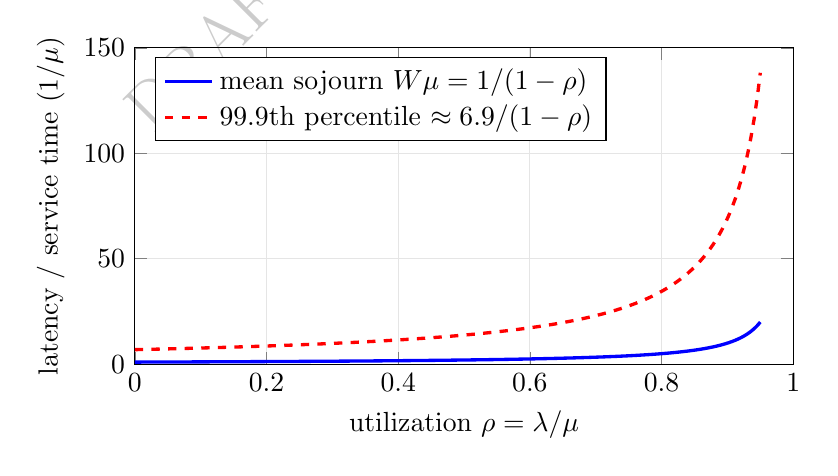
\begin{tikzpicture}
\begin{axis}[
    width=0.82\linewidth, height=5.6cm,
    xlabel={utilization $\rho = \lambda/\mu$},
    ylabel={latency $/$ service time $(1/\mu)$},
    domain=0:0.95, samples=200,
    ymin=0, ymax=150, xmin=0, xmax=1,
    legend pos=north west, legend cell align=left,
    grid=both, grid style={gray!20},
    every axis plot/.append style={very thick},
]
\addplot[blue] {1/(1-x)};
\addlegendentry{mean sojourn $W\mu = 1/(1-\rho)$}
\addplot[red,dashed] {6.9078/(1-x)};
\addlegendentry{$99.9$th percentile $\approx 6.9/(1-\rho)$}
\end{axis}
\end{tikzpicture}
\caption{Latency versus utilization for an M/M/1 servicing stage, in units of the
mean service time $1/\mu$. Both the mean and every tail quantile diverge as
$\rho \to 1$; the tail is a fixed multiple of the mean but far larger in absolute
terms. Keeping the queue short means keeping $\rho$ well left of the knee, which
means making the servicing code fast enough to raise $\mu$.}
\label{fig:qcurve}
\end{figure}

The design consequence is direct. The only free parameters are $\lambda$ and
$\mu$. The arrival rate $\lambda$ --- the market's message rate --- is not ours
to set. The service rate $\mu$ is: it is the reciprocal of the time the servicing
code takes per message. Halving the per-message service time doubles $\mu$,
which for a fixed $\lambda$ moves $\rho$ from, say, $0.9$ to $0.45$ and collapses
the tail. This is why the aggregate speed of the queue-servicing code --- not the
latency of any single send --- governs the tail. A single \fs{} that saves tens
of nanoseconds is uninteresting in isolation; it is decisive because, applied
across every hop of the servicing chain, it raises $\mu$ enough to hold $\rho$
far from $1$ and the queue near empty. \fs{} attacks the tail by attacking
$\mu$.

\subsection{A representative HFT pipeline}
\label{sec:hftarch}

Figure~\ref{fig:hftarch} shows the thread architecture of a representative HFT
market-data-to-order pipeline, drawn from the kaspar-hft reference
implementation. CME's MDP~3.0 market data arrives as two redundant multicast
feeds, channel~A and channel~B. The system decomposes into three sections
connected by exactly two cross-thread hops.

\begin{figure}[t]
\centering
\resizebox{\linewidth}{!}{%
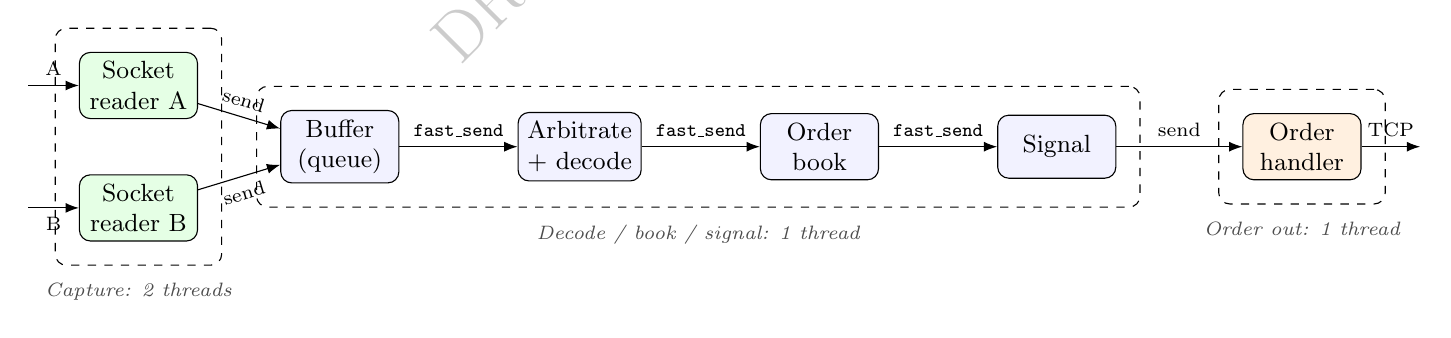
\begin{tikzpicture}[
    font=\small, >=Latex,
    box/.style={draw, rounded corners, minimum height=8mm, minimum width=15mm, align=center, fill=blue!5},
    reader/.style={box, fill=green!10},
    outbox/.style={box, fill=orange!12},
    lbl/.style={font=\scriptsize},
    seclbl/.style={font=\scriptsize\itshape, text=black!70},
]
\node[reader] (sra) {Socket\\reader A};
\node[reader] (srb) [below=7mm of sra] {Socket\\reader B};
\coordinate (mid) at ($(sra)!0.5!(srb)$);
\node[box] (buf)  [right=18mm of mid] {Buffer\\(queue)};
\node[box] (dec)  [right=15mm of buf] {Arbitrate\\+ decode};
\node[box] (book) [right=15mm of dec] {Order\\book};
\node[box] (sig)  [right=15mm of book] {Signal};
\node[outbox] (om)   [right=16mm of sig] {Order\\handler};

% incoming feeds
\draw[->] ($(sra)+(-14mm,0)$) -- node[lbl,above]{A} (sra);
\draw[->] ($(srb)+(-14mm,0)$) -- node[lbl,below]{B} (srb);
% async sends into the buffer (context switch)
\draw[->] (sra) -- node[lbl,sloped,above]{send} (buf);
\draw[->] (srb) -- node[lbl,sloped,below]{send} (buf);
% fast_send chain (single thread)
\draw[->] (buf)  -- node[lbl,above]{\texttt{fast\_send}} (dec);
\draw[->] (dec)  -- node[lbl,above]{\texttt{fast\_send}} (book);
\draw[->] (book) -- node[lbl,above]{\texttt{fast\_send}} (sig);
% async send out (context switch)
\draw[->] (sig)  -- node[lbl,sloped,above]{send} (om);
\draw[->] (om) -- node[lbl,above]{TCP} ($(om)+(15mm,0)$);

\begin{scope}[on background layer]
\node[draw,dashed,rounded corners,fit=(sra)(srb),inner sep=3mm] (s1) {};
\node[draw,dashed,rounded corners,fit=(buf)(dec)(book)(sig),inner sep=3mm] (s2) {};
\node[draw,dashed,rounded corners,fit=(om),inner sep=3mm] (s3) {};
\end{scope}
\node[seclbl,below=1mm of s1.south] {Capture: 2 threads};
\node[seclbl,below=1mm of s2.south] {Decode / book / signal: 1 thread};
\node[seclbl,below=1mm of s3.south] {Order out: 1 thread};
\end{tikzpicture}%
}
\caption{Thread architecture of a representative HFT pipeline. The only
cross-thread hops --- and hence the only context switches --- on the critical
path are the two asynchronous \snd{}s (reader$\to$buffer and
signal$\to$order-handler); each such hop is the expensive operation, measured at
$\sim\!3.4\,\mu$s per round trip (Table~\ref{tab:transport}), because it wakes
another thread. The entire decode/book/signal servicing chain instead collapses
onto a single thread via \fs{}, each hop costing $\sim\!30$~ns --- more than two
orders of magnitude less (see Table~\ref{tab:transport}) --- so it incurs no queue and no context switch. That servicing
chain is the M/M/1 stage of Section~\ref{sec:qtheory} whose per-message service
time, and hence $\mu$, is set by the aggregate cost of these \fs{}s.}
\label{fig:hftarch}
\end{figure}

\paragraph{Section 1 --- capture (two threads).} One socket-reader actor per
channel does nothing but drain its UDP socket and hand each datagram to the next
stage by an \emph{asynchronous} \snd{}. It must be asynchronous: a reader that
made a synchronous, blocking call would stop draining its socket while the callee
ran and would drop packets under a burst --- defeating the reader's only purpose.
In kaspar-hft the reader pre-allocates message buffers and batches whatever the
socket has available before sending, and its handoff to the buffer stage is an
async \snd{}, never a \fs{}.

\paragraph{Section 2 --- decode, book, and signal (one thread).} The datagrams
land in a buffer actor --- the queue --- whose service handler forwards each
message down the remainder of the chain by \fs{}: arbitration between the A and B
feeds, Simple Binary Encoding decode, order-book construction, and signal
generation all run synchronously, in sequence, on this one thread, with no
intervening queue and no context switch between stages. This is precisely the
chained synchronous execution of Section~\ref{sec:mech}: an $N$-stage chain with
$O(1)$ rather than $O(N)$ context switches. This section is the queue-servicing
code whose per-message time sets $\mu$, and it is where \fs{} earns its keep.

\paragraph{Section 3 --- order out (one thread).} When the signal decides to
act, it hands an order to an order-management actor by an asynchronous \snd{};
that actor performs the TCP/iLink write. This hop is asynchronous by design: the
network write takes several microseconds, and blocking the decode-and-book thread
on it would stall servicing of the market-data queue --- driving $\rho$ back
toward $1$, the exact failure the architecture exists to avoid.

\paragraph{Two hops, two switches.} On the critical path from wire to order there
are just two cross-thread hops --- reader$\to$buffer and signal$\to$order-out ---
and therefore two context switches, a fixed cost of a few microseconds in total
\cite{li2007}. Everything between them is collapsed onto a single thread by
\fs{}. The goal is not to remove those two switches; they are cheap and
necessary, because the capture and transmit stages must not block the servicing
stage. The goal is to make the servicing stage between them fast enough that its
queue never grows --- and that is a statement about $\mu$, which is what \fs{}
raises. The mechanism's contribution is thus best measured not as a per-call
latency but as the service rate it sustains on the servicing chain.

% ---------------------------------------------------------------
\section{Performance analysis}
\label{sec:perf}
% ---------------------------------------------------------------

The synchronous path removes, rather than optimizes, the per-message operations
of the asynchronous path. Table~\ref{tab:elim} summarizes the operations
eliminated for a co-located delivery.

\begin{table}[h]
\centering
\caption{Per-message operations on the asynchronous path and their status on the
synchronous path, for co-located actors. This is an analytical account of work
removed.}
\label{tab:elim}
\small
\begin{tabular}{lcc}
\toprule
Per-message operation & Asynchronous & Synchronous \\
\midrule
Message heap allocations           & 1--3 & 0 request (stack-alloc.), 1 reply \\
Mailbox queue operations           & 2 (enqueue $+$ dequeue) & 0 \\
Scheduler invocations              & 1--2 & 0 \\
Context switches (request/reply)   & 2--4 & 0 \\
Context switches, $N$-actor chain  & $O(N)$ & $O(1)$ \\
\bottomrule
\end{tabular}
\end{table}

Each eliminated item has a concrete cost. A context switch is on the order of
$10^3$--$10^4$ processor cycles and evicts cache and TLB state. Heap allocation
of short-lived messages produces fragmentation and, in managed runtimes,
collection pauses; stack allocation reclaims the message on frame unwind with no
allocator or collector involvement. Removing the mailbox operations removes their
synchronization traffic on the memory bus; quantifying that reduction requires
measurement and is left to future work. The chained-execution
result --- $O(1)$ rather than $O(N)$ context switches across an $N$-actor
synchronous chain --- is the largest structural effect for deep call graphs.

\paragraph{Context: measured cost of the asynchronous path.} To indicate the
magnitude of the overhead the synchronous path targets, the asynchronous
messaging path of the same actor runtime has been measured, in separate work
\cite{batching2026}, at $5.5$ to $13.6$ million round trips per second after
successive batching and memory-pooling optimizations; in the saturated
throughput regime a message costs on the order of $74$~ns, while in the sparse
regime an individual send costs several microseconds ($4$--$7~\mu$s), with
condition-variable wakeups costing $1$--$3~\mu$s each. These are measurements of
the \emph{asynchronous} path and bound the per-message costs that synchronous
delivery removes; they are not measurements of \fs{}. We turn now to direct
microbenchmarks of the synchronous path itself.

\subsection{Microbenchmarks of the C++ implementation}
\label{sec:micro}

Table~\ref{tab:elim} predicts that eliminating each per-message operation
produces a measurable reduction in latency. The framework's C++ microbenchmark
suite measures these steps on a \emph{sequential} round trip --- ping $\to$ pong
$\to$ reply with a single message in flight, so each sample is a latency rather
than a saturated throughput \cite{kasparperf}. The figures below were taken on an
AMD~EPYC~9374F (RHEL~9, \texttt{g++}~15), compiled \texttt{-O3 -march=native}
and pinned with \texttt{taskset} to two cores, reported as the median of three
runs. Absolute values depend on hardware, allocator, thread placement, and turbo
state; the durable result is the \emph{ratio} between rows, each of which
isolates one eliminated operation. The \texttt{steady\_clock} resolution on this
machine quantizes to $\sim\!10$~ns, so a per-sample \fs{} percentile is
resolution-bound; \fs{} costs are therefore also reported as amortized ns (total
wall time over $N$ operations, a single clock-read pair), which resolves costs
below one tick.

Table~\ref{tab:transport} isolates the cost of crossing threads; the two
paragraphs that follow it decompose the internal overhead of \fs{} and the
effect of the memory pool.

\paragraph{The cost is thread-crossing, not messaging.} Table~\ref{tab:transport}
holds the work constant --- one ping/pong round trip with a reply --- and varies
only the delivery mechanism, so each row adds back one operation. A cross-thread
asynchronous \snd{} between two actors on separate cores costs $\approx 3.4\,\mu$s
at the median. This cost is dominated by the two cross-core mailbox wakeups per
round trip, each a mutex acquisition and a condition-variable signal on which the
receiving thread must be scheduled; it is placement-sensitive, because the
cross-core path depends on which cores the two threads occupy. Co-scheduling the
two actors on one thread (grouping) removes both wakeups and reduces the round
trip to $90$~ns, a $37\times$ reduction. Replacing the remaining mailbox push/pop
with an inline \fs{} reduces it to $\sim\!30$~ns (amortized; the per-sample $p50$
is resolution-bound), because a \fs{} is mechanically a locked function call: it
takes the receiver's lock and runs the handler inline. Measured the same way, a
bare direct call costs $\sim\!1$~ns, so \fs{} adds $\sim\!10$~ns over a direct
call --- covering the receiver-lock acquire/release, message-field setup,
handler-cache dispatch, and reply wrapping.

\begin{table}[!htb]
\centering
\caption{\textbf{The cost is thread-crossing, not messaging.} Same ping/pong
round trip with a reply; only the delivery mechanism varies. Each row eliminates
one operation relative to the row above. ``Thread hop'' is a cross-core mailbox
wakeup (mutex $+$ condition variable); ``queue'' is a mailbox push/pop.
The $p50$ column is per-sample round-trip latency; the \fs{} figure is
amortized, because its per-sample $p50$ is resolution-bound (the
\texttt{steady\_clock} tick is $\sim\!10$~ns), and its speedup is computed on
amortized figures. The grouped and \fs{} rows show negligible spread.}
\label{tab:transport}
\small
\begin{tabular}{lccccr}
\toprule
Delivery mode & Threads & Thread hop & Queue & $p50$ RT (ns) & Speedup \\
\midrule
\snd{}, ungrouped        & 2 & yes & yes & $\sim\!3370$  & $1\times$ \\
\snd{}, grouped          & 1 & no  & yes & $90$          & $37\times$ \\
\fs{} (inline)           & 1 & no  & no  & $\sim\!30$    & $\sim\!110\times$ \\
\bottomrule
\end{tabular}
\end{table}

\paragraph{Grouping, and why \fs{} improves on it.} The grouped row is the
strongest conventional alternative. The framework places a set of actors in a
\texttt{Group}, co-scheduled on a single thread behind a single mailbox, so an
asynchronous \snd{} within the group never crosses a core: it is a push and a pop
on a queue owned by the running thread. This is the standard low-latency actor
optimization --- same-thread messaging in Actor4j, a shared dispatcher in Akka
(Section~\ref{sec:survey}) --- and it reduces the round trip from $\sim\!3.4\,\mu$s
to $90$~ns. Grouping still pays for the queue: the message is enqueued, the run
loop dequeues it, and the handler runs on a later turn. \fs{} removes that layer.
On the same thread it does not enqueue; it takes the receiver's lock and runs the
handler inline, returning the reply as a value, in $\sim\!30$~ns --- about
$3\times$ faster than grouping. Grouping removes the thread hop; \fs{} removes the
thread hop \emph{and} the queue. This synchronous, inline, receiver-transparent
delivery is, to our knowledge, absent from the mainstream actor systems surveyed
in Section~\ref{sec:survey}. The intended use follows: group the actors of a
servicing stage onto one thread and drive them with \fs{}, so that an $N$-actor
pipeline collapses to a single inline call chain (the middle section of
Figure~\ref{fig:hftarch}).

\paragraph{Allocation, not dispatch, is the only variable cost.} Beyond the
inline dispatch, the only per-message cost a caller pays is for memory it chooses
to allocate. A request message kept on the stack requires none, because \fs{}
blocks until the handler returns (Section~\ref{sec:mech}). For a message that must
outlive the call, allocation from a \texttt{MemoryPool} replaces a general-purpose
\texttt{new}/\texttt{delete}. On a grouped-\snd{} round trip with two allocations,
the pool reduces the amortized cost from $\sim\!128$~ns (pool off) to $\sim\!92$~ns
(pool on). The larger and platform-independent benefit is the tail: in a separate
run the maximum round trip fell from $5.5$~ms to $33\,\mu$s once pooled, because
the pool never takes the general allocator's occasional slow path. This is the
quantity that matters for Section~\ref{sec:queueing}: a two-order-of-magnitude
reduction of the $p99.9{+}$ tail that a slow servicing stage feeds into a growing
queue.

\paragraph{Scope.} These are sequential latencies with one message in flight, not
saturated throughput, and they do not vary contention or chain depth. The
established results are: \fs{} costs tens of nanoseconds; its overhead over a
direct call is $\sim\!10$~ns plus whatever memory the caller allocates; it
improves on same-thread grouping by about $3\times$; and pooling removes the
latency tail. The multi-axis, saturated evaluation (Section~\ref{sec:disc})
remains future work.

\subsection{Mailbox queue types and their selection}
\label{sec:qtypes}

The mailbox is a \texttt{std::variant} over four multi-producer/single-consumer
queue implementations, selectable per actor: \texttt{BQueue} (a mutex and
condition variable around a ring buffer); \texttt{BQueueBatched} (the same lock,
but the consumer drains the whole queue under one acquisition); \texttt{ShardedBQueue}
($N$ independent lanes, each separately locked, joined by an atomic cursor); and
\texttt{LockFreeMPSC} (a bounded lock-free Vyukov ring, in which a producer
reserves a slot with a single atomic operation). Because the variant holds the
concrete type, \texttt{push} and the drain loop are devirtualized and inlined.
Table~\ref{tab:qtypes} measures the four on the EPYC target across the three
regimes that separate them; a fourth regime, a single cross-thread message,
distinguishes none of them, because thread placement moves the figure by
$2.2\times$ --- more than the gap between queues.

\begin{table}[!htb]
\centering
\caption{\textbf{Four mailbox queue types, one column per distinguishing regime}
(EPYC target, pinned, median of three runs). \emph{Grouped}: single-thread
round-trip median. \emph{Burst}: single bursty producer, amortized cost per
message. \emph{Fan-in}: 32 concurrent producers, push $p99$. Bold marks the best
in each regime; no type is best in all three.}
\label{tab:qtypes}
\small
\begin{tabular}{lrrr}
\toprule
Queue type & Grouped $p50$ (ns) & Burst (ns/msg) & Fan-in $p99$ ($\mu$s) \\
\midrule
\texttt{BQueue}        & $90$          & $605.8$          & $69.9$ \\
\texttt{BQueueBatched} & $90$          & $\mathbf{584.9}$ & $72.4$ \\
\texttt{ShardedBQueue} & $190$         & $983.1$          & $\mathbf{6.6}$ \\
\texttt{LockFreeMPSC}  & $\mathbf{70}$ & $672.0$          & $16.5$ \\
\bottomrule
\end{tabular}
\end{table}

No single queue wins everywhere. On a shared (grouped) thread, \texttt{LockFreeMPSC}
has the lowest median ($70$~ns, $1.3\times$ below \texttt{BQueue}), because its
push and pop are each an uncontended atomic operation with no lock or wakeup.
Under a bursty single producer --- the market-data regime of the case study ---
\texttt{BQueueBatched} is fastest ($584.9$~ns/msg): draining an entire packet
burst under one lock acquisition amortizes the lock over the burst, and
\texttt{BQueue} trails by under $4\%$. Under 32-producer fan-in, \texttt{ShardedBQueue}
wins decisively --- $p99$ of $6.6~\mu$s against \texttt{BQueue}'s $69.9~\mu$s
($10.6\times$), and $3.6\times$ the throughput --- because its independent lanes
remove the single-mutex serialization that dominates the other three; it pays for
those lanes in the other regimes, where it is the slowest of the four.

The selection rule follows. Default every actor to \texttt{BQueue}: it is fastest
or within a few percent in every regime except fan-in, and it has the most stable
tail of the four (grouped \texttt{max} $2.4$--$9~\mu$s, versus $14$--$16~\mu$s for
\texttt{LockFreeMPSC}). Override to \texttt{ShardedBQueue} only for the few actors
written to by many producers concurrently --- a shared order-out actor, or a
fan-in aggregator across market-data handlers --- the one regime in which it wins.
\texttt{LockFreeMPSC}, despite the best grouped median, is not recommended as a
default because its tail is the least stable measured; \texttt{ShardedBQueue} is
not a default because its lanes are wasted, and counterproductive, outside fan-in.

\FloatBarrier

% ---------------------------------------------------------------
\section{Case study: tick-to-book latency in a live market-data path}
\label{sec:casestudy}
% ---------------------------------------------------------------

The microbenchmarks of Section~\ref{sec:micro} measure the framework's
per-message cost in isolation, and the queueing analysis of
Section~\ref{sec:queueing} predicts, in principle, where latency comes from. This
section grounds both in a live measurement of the \textsc{kaspar-hft}
market-data path on production exchange data, and asks the paper's title question
directly: is the actor model's overhead small enough for a high-frequency
market-data path? The measurements below are drawn from a companion latency study
of the same system \cite{mdlatency2026}.

\subsection{Setup}

The path under measurement is the market-data ingest of Section~\ref{sec:hftarch}:
read a UDP datagram off CME MDP~3.0 multicast, decode the Simple Binary Encoding
(SBE) messages \cite{fixsbe} inside it, apply them to an order book, and publish.
Two timestamps are taken per message --- $t_0$ when the datagram comes up from the
socket, $t_1$ when the book update is published --- and their difference is
recorded for every message. Structurally this is two actor stages: a socket-reader
actor hands each datagram to a decode-and-order-book actor by an asynchronous
\snd{} (necessarily asynchronous --- a blocking reader would stop draining its
socket and drop packets), and decode plus book construction run together on the
second thread. The handoff between the two stages is the decoder's mailbox --- a
bounded ring buffer of datagrams (a \texttt{BQueue}) --- and we write
$\text{qlen}$ for its occupancy: the number of datagrams already
waiting in the ring when a given datagram is handed to the decoder, so
$\text{qlen}=0$ means the ring was empty and the datagram was picked up at once.
This is the ``ring'' and the ``queue'' referred to throughout this section. The
handoff is a single bursty producer, the regime in which \texttt{BQueueBatched}
is marginally faster than the \texttt{BQueue} used here (Section~\ref{sec:qtypes});
the difference is a few percent of the mailbox cost and negligible against the
$\sim\!7~\mu$s floor.
Three instruments (E-mini S\&P~500, ES; E-mini Nasdaq-100, NQ;
10-year Treasury Note, ZN), each with a book-update and a trade stream:
$8.29$~million messages over 53 minutes of a busy afternoon
(2026-09-16). One caveat bounds everything below: $t_0$ is a \emph{software}
timestamp taken at the socket read, so time spent in the NIC and the kernel is
excluded. This is socket-to-book, not wire-to-book.

\subsection{The per-message model: floor plus serialization}
\label{sec:floorslope}

One UDP datagram carries many SBE messages, decoded in order. Write $\text{idx}$
for a message's position within its packet, counted from zero: $\text{idx}=0$ is
the message decoded first, $\text{idx}=1$ the next, and so on. A message at
position $\text{idx}$ therefore waits for the $\text{idx}$ decodes ahead of it
before its own runs --- a wait that sits inside its measured latency, and that is
zero exactly when $\text{idx}=0$. Restricting to messages that arrive to an empty
ring (nothing queued ahead of their packet), so the only remaining wait is
in-packet, the median latency is linear in $\text{idx}$,
\[
  \text{median latency} \;\approx\; \text{floor} \;+\; \text{slope}\times\text{idx},
\]
with the two coefficients of Table~\ref{tab:floorslope}, fitted on medians. (Means
are useless here: a single multi-millisecond stall in a cell moves the mean by
tens of microseconds, so every quantity in this section is a median or a
percentile.) The two coefficients carry the argument.

The \emph{floor} --- the intercept, a message first in its packet --- agrees to
within $0.42~\mu$s across six independent streams, $6.8$--$7.2~\mu$s. It is the
irreducible cost of decoding one SBE message and applying it to the book; it is
insensitive to queue length; and it is stable under
load, moving by at most $+0.4~\mu$s (and \emph{falling} on two of three
instruments) during a Federal Reserve release that raised the packet rate
$4.6$--$9.8\times$ in a second. Against this $\sim\!7~\mu$s floor the framework's
per-message contribution --- the mailbox handoff and dispatch of
Section~\ref{sec:micro} --- is tens of nanoseconds: a \fs{} dispatch is
$\sim\!30$~ns. \emph{The actor abstraction is under $1\%$ of the floor}; the floor
is SBE decode and book mutation, not message delivery.

The \emph{slope} --- the per-message serialization cost, $0.31$--$0.97~\mu$s ---
determines the tail. In-packet position scales linearly into latency: the last
message of a $45$-message packet incurs $44\times0.57 \approx 25~\mu$s on top of
the floor, deterministically. On the trade streams a message is essentially never alone
($99.3$--$99.6\%$ have another message ahead of them in the same packet), which is
why the trade medians already sit above the book medians. Shaving $100$~ns off the
floor moves every message by $100$~ns; shaving it off the slope moves a message by
$\text{idx}\times100$~ns, and $\text{idx}$ is exactly what is large in the tail.
The design lever is the slope --- not the floor, and not the mailbox queue, which
is rare: between $87\%$ and $99.7\%$ of messages arrive to find the ring empty.

\begin{table}[t]
\centering
\caption{The per-message model
$\text{median}\approx\text{floor}+\text{slope}\times\text{idx}$, fitted on medians
at queue length zero. The floor (a message first in its packet) agrees within
$0.42~\mu$s across six streams; the slope (the in-packet serialization cost)
varies $\sim\!3\times$ and is where the tail is bought.}
\label{tab:floorslope}
\small
\begin{tabular}{lrr}
\toprule
Stream & Floor ($\mu$s) & Slope (ns/msg) \\
\midrule
ES book  & 6.98 & 566 \\
NQ book  & 7.23 & 312 \\
ZN book  & 6.83 & 966 \\
ES trade & 6.81 & 714 \\
NQ trade & 7.14 & 526 \\
ZN trade & 6.81 & 965 \\
\bottomrule
\end{tabular}
\end{table}

\begin{figure}[t]
\centering
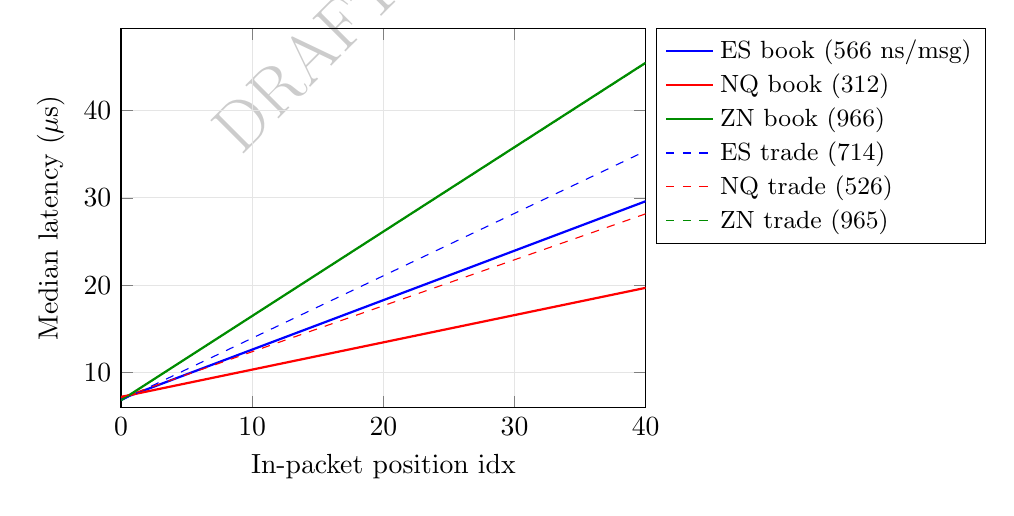
\begin{tikzpicture}
\begin{axis}[
  width=0.68\linewidth, height=6.4cm,
  xlabel={In-packet position idx}, ylabel={Median latency ($\mu$s)},
  domain=0:40, samples=2,
  xmin=0, xmax=40, ymin=6,
  legend style={at={(1.02,1)},anchor=north west,font=\small},
  legend cell align=left,
  grid=both, grid style={gray!20},
]
\addplot[blue,thick]           {6.98+0.566*x}; \addlegendentry{ES book (566 ns/msg)}
\addplot[red,thick]            {7.23+0.312*x}; \addlegendentry{NQ book (312)}
\addplot[green!55!black,thick] {6.83+0.966*x}; \addlegendentry{ZN book (966)}
\addplot[blue,dashed]          {6.81+0.714*x}; \addlegendentry{ES trade (714)}
\addplot[red,dashed]           {7.14+0.526*x}; \addlegendentry{NQ trade (526)}
\addplot[green!55!black,dashed] {6.81+0.965*x}; \addlegendentry{ZN trade (965)}
\end{axis}
\end{tikzpicture}
\caption{The per-message model $\text{median}=\text{floor}+\text{slope}\times
\text{idx}$ (Table~\ref{tab:floorslope}), one line per stream. All six share a
$\sim\!7~\mu$s floor at $\text{idx}=0$; the slope --- the per-message
serialization cost --- sets the divergence, from $312$~ns/msg (NQ~book) to
$966$~ns/msg (ZN~book).}
\label{fig:floorslope}
\end{figure}

\subsection{Three estimates of the floor}
\label{sec:floor-robust}

The floor of Table~\ref{tab:floorslope} is a fitted intercept. Two further
estimates, constructed differently, agree with it. The first isolates the hot path
directly: the subset of messages with $\text{qlen}=0$ and $\text{idx}=0$, for which
neither the queue nor in-packet serialization contributes, so its median is the
floor with no model interposed (Table~\ref{tab:floordirect}). Across six streams
the spread is $1.41~\mu$s; across the three book streams it is $0.35~\mu$s.

\begin{table}[!htb]
\centering
\caption{\textbf{Direct hot-path floor:} median latency of the subset at
$\text{qlen}=0$ and $\text{idx}=0$, with the sample size. No queue and no in-packet
serialization contribute to these messages.}
\label{tab:floordirect}
\small
\begin{tabular}{lrr}
\toprule
Stream & Median ($\mu$s) & $n$ \\
\midrule
ES book  & 7.01 & 1{,}781{,}767 \\
NQ book  & 7.24 & 1{,}841{,}447 \\
ZN book  & 6.89 & \phantom{0,}671{,}271 \\
ES trade & 7.62 & \phantom{0,00}1{,}008 \\
NQ trade & 8.30 & \phantom{0,000,}298 \\
ZN trade & 7.96 & \phantom{0,000,}474 \\
\bottomrule
\end{tabular}
\end{table}

The second estimate is the fitted $\text{idx}=0$ intercept of the median ladder
(Table~\ref{tab:floorslope}). The third is measured during the Federal Open Market
Committee statement, when the packet rate rose $6.5\times$, $4.6\times$, and
$9.8\times$ on the three instruments within a second; taking the floor from
single-message packets ($\text{span}\approx1$) in that window gives the third row
of Table~\ref{tab:floor3}. The three agree to within a few tenths of a
microsecond.

\begin{table}[!htb]
\centering
\caption{\textbf{Three independent estimates of the floor} ($\mu$s), book streams.
The three methods differ in their sample, their estimator, and the load regime
they were taken under, and agree to within $0.4~\mu$s.}
\label{tab:floor3}
\small
\begin{tabular}{lrrr}
\toprule
Method & ES & NQ & ZN \\
\midrule
Direct median ($\text{qlen}=0$, $\text{idx}=0$)        & 7.01 & 7.24 & 6.89 \\
Fitted $\text{idx}=0$ intercept (median ladder)        & 6.98 & 7.23 & 6.83 \\
Floor at $\text{span}\approx 1$ during the FOMC release & 7.1\phantom{0} & 7.5\phantom{0} & 7.0\phantom{0} \\
\bottomrule
\end{tabular}
\end{table}

The third estimate is the informative one. During the release the floor moved by
at most $+0.4~\mu$s, and fell on two of the three instruments. The hot path is not
rate-sensitive: three methods, three instruments, all within $6.8$--$7.5~\mu$s.
This is the most stable quantity in the study --- it moved negligibly when the
sample tripled, when the estimator changed from mean to median, and when the
packet rate rose tenfold.

\subsection{The distribution and its tail}

The median is not the quantity a trading operation is judged on; the tail is.
Table~\ref{tab:mddist} gives the unconditional distribution. The medians cluster
--- three separate multicast channels, three instruments, all within $0.2~\mu$s
--- but the tails come apart: ES book's $p99$ is $18.5~\mu$s, ZN book's is
$57.0~\mu$s, and ZN trade's is $219~\mu$s. Expressed as amplification from median
to $p99$, the streams range from $1.9\times$ (NQ book) to $14.2\times$ (ZN
trade). A single ``$8~\mu$s'' figure for this system would be true and would say
nothing about the quantity that matters.

\begin{table}[t]
\centering
\caption{Unconditional socket-to-book latency distribution ($\mu$s), every
admitted message per stream, no conditioning. The median is uniform across
streams; the tail is not.}
\label{tab:mddist}
\small
\begin{tabular}{lrrrrrr}
\toprule
Stream & Messages & $p50$ & $p90$ & $p99$ & $p99.9$ & max \\
\midrule
ES book  & 2{,}861{,}519 & 7.1 & 10.6 & 18.5 & 41.2 & 1148.4 \\
NQ book  & 3{,}792{,}033 & 7.3 & \phantom{0}9.9 & 13.6 & 24.7 & 5567.0 \\
ZN book  & 1{,}119{,}746 & 7.1 & 12.1 & 57.0 & 180.9 & 2458.2 \\
ES trade & \phantom{0,}296{,}736 & 9.0 & 15.3 & 38.0 & 127.7 & \phantom{0}421.5 \\
NQ trade & \phantom{0,}110{,}003 & 8.3 & 12.5 & 31.2 & 83.7 & \phantom{0}694.2 \\
ZN trade & \phantom{0,}114{,}154 & 15.4 & 69.3 & 219.4 & 409.5 & \phantom{0}504.8 \\
\bottomrule
\end{tabular}
\end{table}

\begin{figure}[t]
\centering
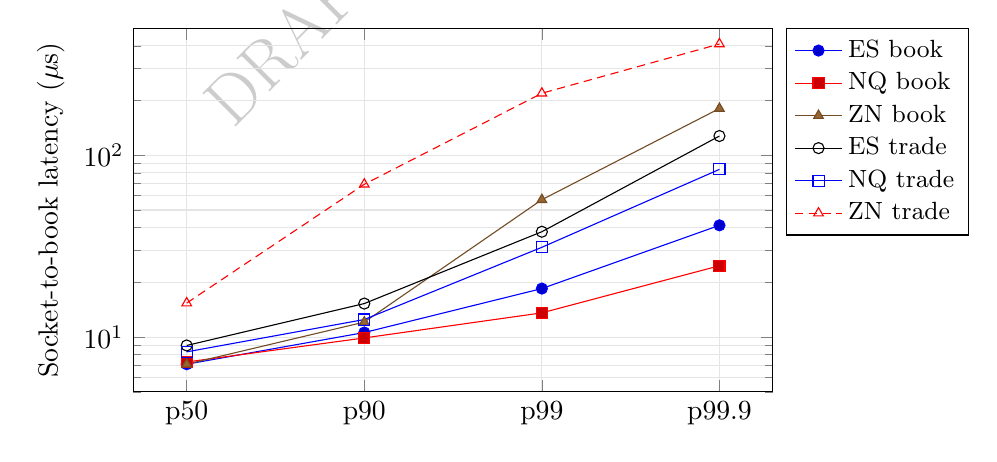
\begin{tikzpicture}
\begin{axis}[
  width=0.8\linewidth, height=6.2cm,
  ymode=log, log basis y=10,
  symbolic x coords={p50,p90,p99,p99.9},
  xtick=data, ymin=5, ymax=500,
  ylabel={Socket-to-book latency ($\mu$s)},
  legend style={at={(1.02,1)},anchor=north west,font=\small},
  legend cell align=left, enlarge x limits=0.1,
  grid=both, grid style={gray!20},
]
\addplot+[mark=*]         coordinates {(p50,7.1)(p90,10.6)(p99,18.5)(p99.9,41.2)};  \addlegendentry{ES book}
\addplot+[mark=square*]   coordinates {(p50,7.3)(p90,9.9)(p99,13.6)(p99.9,24.7)};   \addlegendentry{NQ book}
\addplot+[mark=triangle*] coordinates {(p50,7.1)(p90,12.1)(p99,57.0)(p99.9,180.9)}; \addlegendentry{ZN book}
\addplot+[mark=o]         coordinates {(p50,9.0)(p90,15.3)(p99,38.0)(p99.9,127.7)}; \addlegendentry{ES trade}
\addplot+[mark=square]    coordinates {(p50,8.3)(p90,12.5)(p99,31.2)(p99.9,83.7)};  \addlegendentry{NQ trade}
\addplot+[mark=triangle]  coordinates {(p50,15.4)(p90,69.3)(p99,219.4)(p99.9,409.5)}; \addlegendentry{ZN trade}
\end{axis}
\end{tikzpicture}
\caption{Socket-to-book latency percentiles per stream (Table~\ref{tab:mddist}),
log scale. Medians cluster near $7$--$15~\mu$s; the tails diverge, ZN~trade
reaching $219~\mu$s at $p99$ and $410~\mu$s at $p99.9$.}
\label{fig:mddist}
\end{figure}

The tail is set by the in-packet serialization of Section~\ref{sec:floorslope},
not by the framework: a message's latency is floor plus slope times its position,
and a bursty feed produces long packets, so the tail is that slope multiplied by a
large position.

\subsection{Isolating the queue from packet position}
\label{sec:queue-deconf}

The floor-plus-slope model of Section~\ref{sec:floorslope} and the distribution of
Table~\ref{tab:mddist} both aggregate over queue occupancy. Grouping latency by
$\text{qlen}$ and reporting a within-group statistic measures the queue only if
nothing else varies across the groups. Something does: a burst that fills the ring
tends also to produce larger packets, so a message at high $\text{qlen}$ also sits,
on some streams, deeper inside its own packet. Part of the rise a naive
$\text{qlen}$ table attributes to the queue is therefore in-packet position. The
correction is the move of Section~\ref{sec:floorslope} applied again: hold
$\text{idx}=0$, so the message is first in its packet and no in-packet
serialization remains in its latency, and vary $\text{qlen}$. Whatever still moves
is the queue.

\paragraph{Estimator.} Within a $\text{qlen}$ cell the \emph{mean} is not a measure
of the queue. A cell may hold tens of messages, and a single multi-millisecond
stall moves the mean by tens of microseconds: on one cut NQ~book's mean at
$\text{qlen}=0$ was $280~\mu$s against a median of $7.4~\mu$s. Stalls are a
separate phenomenon; every figure in this section is a median or a percentile.

\paragraph{Columns.} Tables~\ref{tab:deconf-es}--\ref{tab:deconf-trade} carry
eleven columns. \emph{qlen} is the number of packets already in the ring when this
message's packet was handed to the consumer. \emph{msgs} is the count at that
queue length --- the denominator for the pooled quantiles, and it collapses
quickly (ES~book has $2.66$~million messages at $\text{qlen}=0$ and $51$ at
$\text{qlen}=6$). \emph{med}, \emph{$p90$}, \emph{$p99$} are the latency quantiles
pooled over in-packet position; these are the confounded columns and form an upper
bound on the queue's cost. \emph{span} is the mean packet size (SBE messages per
datagram) of those messages --- the suspected confounder --- and \emph{idx} their
mean in-packet position, which is approximately $\text{span}/2$. \emph{$n_0$} is
the subset first in their own packet, the deconfounded sample; \emph{med$_0$},
\emph{$p90_0$}, \emph{$p99_0$} are the quantiles of that subset, with the bracketed
figure in med$_0$ the change from the $\text{qlen}=0$ row. Percentiles are
suppressed (\,--\,) where $n_0$ is below roughly $200$, at which point a $99$th
percentile is the largest sample rather than a measurement.

\begin{table}[htbp]
\centering
\caption{\textbf{ESZ6 book: queue occupancy versus latency, deconfounded from
packet position.} Latencies in $\mu$s. Pooled quantiles (med, $p90$, $p99$) run
over all in-packet positions; span/idx are the mean packet size and in-packet
position; $n_0$ and the $_0$ quantiles are the subset first in their packet
($\text{idx}=0$). Bracketed: change in med$_0$ from $\text{qlen}=0$.}
\label{tab:deconf-es}
\resizebox{\textwidth}{!}{%
\begin{tabular}{rrrrrrrrrrr}
\toprule
qlen & msgs & med & $p90$ & $p99$ & span & idx & $n_0$ & med$_0$ & $p90_0$ & $p99_0$ \\
\midrule
0 & 2{,}664{,}628 & 7.1 & 10.4 & 17.9 & 2.20 & 0.62 & 2{,}303{,}948 & 6.9 & 9.8 & 13.9 \\
1 & 181{,}719 & 6.5 & 12.3 & 24.2 & 1.78 & 0.39 & 162{,}136 & 6.3 ($-$0.6) & 11.4 & 17.9 \\
2 & 12{,}790 & 7.2 & 12.8 & 42.2 & 1.45 & 0.21 & 12{,}175 & 7.1 ($+$0.2) & 12.3 & 22.2 \\
3 & 1{,}619 & 8.6 & 16.5 & 44.6 & 1.20 & 0.06 & 1{,}547 & 8.5 ($+$1.5) & 15.7 & 35.0 \\
4 & 376 & 10.2 & 92.8 & 309.7 & 4.17 & 1.57 & 320 & 9.8 ($+$2.8) & 21.8 & 79.2 \\
5 & 134 & 15.3 & 348.6 & -- & 9.64 & 4.26 & 97 & 11.5 ($+$4.6) & 27.5 & -- \\
6 & 51 & 17.0 & -- & -- & 1.18 & 0.08 & 48 & 16.6 ($+$9.7) & -- & -- \\
7 & 90 & 398.0 & 445.2 & -- & 26.00 & 12.50 & 22 & n/a & -- & -- \\
8 & 41 & 459.7 & -- & -- & 14.46 & 6.73 & 18 & n/a & -- & -- \\
\bottomrule
\end{tabular}}
\end{table}

\begin{table}[htbp]
\centering
\caption{\textbf{NQZ6 book: queue occupancy versus latency, deconfounded.}
Columns as in Table~\ref{tab:deconf-es}.}
\label{tab:deconf-nq}
\resizebox{\textwidth}{!}{%
\begin{tabular}{rrrrrrrrrrr}
\toprule
qlen & msgs & med & $p90$ & $p99$ & span & idx & $n_0$ & med$_0$ & $p90_0$ & $p99_0$ \\
\midrule
0 & 3{,}310{,}403 & 7.4 & 9.9 & 13.5 & 2.40 & 0.80 & 2{,}586{,}119 & 7.2 & 9.5 & 12.4 \\
1 & 463{,}440 & 6.1 & 9.0 & 13.6 & 2.11 & 0.58 & 371{,}010 & 5.9 ($-$1.3) & 8.6 & 12.9 \\
2 & 15{,}274 & 7.0 & 11.6 & 25.8 & 1.92 & 0.36 & 13{,}508 & 6.9 ($-$0.3) & 11.4 & 20.5 \\
3 & 1{,}641 & 8.6 & 17.8 & 168.5 & 2.82 & 0.79 & 1{,}457 & 8.3 ($+$1.1) & 14.3 & 34.3 \\
4 & 340 & 12.1 & 91.8 & 456.4 & 3.39 & 1.17 & 276 & 11.2 ($+$4.0) & 27.6 & 456.4 \\
5 & 121 & 17.7 & 384.8 & -- & 1.39 & 0.21 & 109 & 16.4 ($+$9.2) & 382.0 & -- \\
6 & 72 & 16.8 & 393.5 & -- & 1.19 & 0.12 & 64 & 16.8 ($+$9.5) & 414.5 & -- \\
7 & 57 & 19.4 & -- & -- & 1.51 & 0.35 & 46 & 22.8 ($+$15.5) & -- & -- \\
8 & 36 & 95.4 & -- & -- & 2.06 & 0.50 & 29 & n/a & -- & -- \\
9 & 42 & 74.0 & -- & -- & 1.95 & 0.55 & 34 & 67.7 ($+$60.5) & -- & -- \\
\bottomrule
\end{tabular}}
\end{table}

\begin{table}[htbp]
\centering
\caption{\textbf{ZNZ6 book: queue occupancy versus latency, deconfounded.}
Columns as in Table~\ref{tab:deconf-es}. ZN is the stream whose packets grow with
queue length; compare med and med$_0$.}
\label{tab:deconf-zn}
\resizebox{\textwidth}{!}{%
\begin{tabular}{rrrrrrrrrrr}
\toprule
qlen & msgs & med & $p90$ & $p99$ & span & idx & $n_0$ & med$_0$ & $p90_0$ & $p99_0$ \\
\midrule
0 & 988{,}149 & 7.2 & 11.9 & 43.9 & 3.13 & 1.12 & 829{,}350 & 6.9 & 10.2 & 15.4 \\
1 & 124{,}649 & 6.3 & 12.6 & 88.8 & 3.41 & 1.22 & 105{,}162 & 6.0 ($-$0.9) & 9.4 & 17.0 \\
2 & 4{,}831 & 10.8 & 97.3 & 266.6 & 12.02 & 5.49 & 2{,}740 & 7.6 ($+$0.7) & 14.2 & 72.8 \\
3 & 1{,}088 & 84.9 & 214.0 & 307.4 & 18.83 & 8.92 & 430 & 9.4 ($+$2.5) & 27.3 & 160.3 \\
4 & 477 & 128.2 & 228.5 & 458.5 & 23.33 & 11.18 & 130 & 11.6 ($+$4.7) & 69.4 & -- \\
5 & 206 & 256.0 & 326.8 & 334.5 & 26.50 & 12.74 & 44 & 21.7 ($+$14.8) & -- & -- \\
6 & 70 & 163.3 & 191.5 & -- & 17.21 & 8.11 & 31 & 18.3 ($+$11.4) & -- & -- \\
7 & 115 & 193.4 & 342.0 & -- & 26.65 & 12.83 & 21 & n/a & -- & -- \\
8 & 50 & 150.2 & -- & -- & 20.56 & 9.78 & 12 & n/a & -- & -- \\
\bottomrule
\end{tabular}}
\end{table}

\begin{table}[htbp]
\centering
\caption{\textbf{Trade streams: queue occupancy versus latency, deconfounded.}
Columns as in Table~\ref{tab:deconf-es}, with a leading stream label. The trade
streams reach $\text{qlen}\ge 1$ on too few messages for the deconfounded subset
to support percentiles.}
\label{tab:deconf-trade}
\resizebox{\textwidth}{!}{%
\begin{tabular}{lrrrrrrrrrrr}
\toprule
stream & qlen & msgs & med & $p90$ & $p99$ & span & idx & $n_0$ & med$_0$ & $p90_0$ & $p99_0$ \\
\midrule
ES & 0 & 295{,}337 & 9.0 & 15.2 & 34.6 & 8.51 & 4.25 & 1{,}522 & 7.9 & 11.2 & 15.7 \\
ES & 1 & 1{,}242 & 10.3 & 128.7 & 202.7 & 22.48 & 11.41 & 14 & n/a & -- & -- \\
ES & 2 & 129 & 144.7 & 216.8 & -- & 57.64 & 28.36 & 2 & n/a & -- & -- \\
\midrule
NQ & 0 & 109{,}541 & 8.3 & 12.5 & 29.6 & 7.06 & 3.63 & 416 & 8.2 & 10.7 & 32.7 \\
NQ & 1 & 387 & 8.5 & 74.7 & 93.9 & 16.07 & 7.91 & 5 & n/a & -- & -- \\
NQ & 2 & 65 & 100.7 & 139.7 & -- & 83.72 & 41.58 & 0 & n/a & -- & -- \\
\midrule
ZN & 0 & 108{,}706 & 15.0 & 61.0 & 142.4 & 32.03 & 16.00 & 649 & 8.4 & 62.9 & 111.4 \\
ZN & 1 & 4{,}213 & 50.5 & 191.2 & 285.9 & 30.68 & 15.28 & 107 & 76.8 ($+$68.4) & 170.5 & -- \\
ZN & 2 & 755 & 219.5 & 385.0 & 415.2 & 71.95 & 36.29 & 9 & n/a & -- & -- \\
ZN & 3 & 139 & 234.8 & 259.5 & -- & 68.78 & 39.65 & 2 & n/a & -- & -- \\
\bottomrule
\end{tabular}}
\end{table}

\paragraph{The queue is convex.} Reading med$_0$ down each book stream isolates
the queue with position held at zero. ES: $6.9, 6.3, 7.1, 8.5, 9.8, 11.5,
16.6~\mu$s, successive increments $-0.6, +0.8, +1.4, +1.3, +1.7, +5.1$. NQ:
increments $-1.3, +1.0, +1.4, +2.9, +5.2$. ZN: $-0.9, +1.6, +1.8, +2.2, +10.1$.
Three independent multicast channels give three convex curves with the confounder
held fixed --- the shape the M/M/1 model of Section~\ref{sec:queueing} predicts.

\paragraph{The convexity is concentrated in the tail.} The queue's effect on the
median is small; its effect on the upper percentiles is roughly an order of
magnitude larger. Table~\ref{tab:deconf-ratios} gives the ratio from
$\text{qlen}=0$ to $\text{qlen}=3$ at each quantile. With position held at zero,
three queued packets cost ES $+1.5~\mu$s at the median but $+21~\mu$s at $p99$, and
ZN $+145~\mu$s at $p99$. The pooled columns --- every message at that queue length,
whatever its packet position, the figure an operator experiences --- are larger
again, and diverge from the deconfounded ratios exactly where packets grow with
queue length: on ES the two agree (ES packets do not grow with $\text{qlen}$), on
ZN they do not.

\begin{table}[htbp]
\centering
\caption{\textbf{Queue cost from $\text{qlen}=0$ to $\text{qlen}=3$, as a ratio at
each quantile.} Left: position held at $\text{idx}=0$ (queue only). Right: pooled
over in-packet position (queue $+$ packet, as experienced). The two agree on ES,
where packets do not grow with queue length, and diverge on ZN, where they do.}
\label{tab:deconf-ratios}
\small
\begin{tabular}{lrrr@{\hspace{2.4em}}rrr}
\toprule
& \multicolumn{3}{c}{At $\text{idx}=0$} & \multicolumn{3}{c}{Pooled over idx} \\
\cmidrule(lr){2-4}\cmidrule(l){5-7}
Stream & $p50$ & $p90$ & $p99$ & $p50$ & $p90$ & $p99$ \\
\midrule
ES book & $1.23\times$ & $1.60\times$ & $2.52\times$ & $1.21\times$ & $1.59\times$ & $2.49\times$ \\
NQ book & $1.15\times$ & $1.51\times$ & $2.77\times$ & $1.16\times$ & $1.80\times$ & $12.48\times$ \\
ZN book & $1.36\times$ & $2.68\times$ & $10.41\times$ & $11.79\times$ & $17.98\times$ & $7.00\times$ \\
\bottomrule
\end{tabular}
\end{table}

\paragraph{Frequency.} The effect is confined to a rare event. ES~book reaches
$\text{qlen}\ge 3$ on $2{,}311$ of $2{,}861{,}519$ messages, $0.08\%$. The queue is
a large effect at the percentiles on a small fraction of messages, not a small
effect everywhere.

\paragraph{Packet growth splits the streams.} The \emph{span} column separates two
regimes. On ZN, packets grow as the ring fills --- ZN~book runs $3.13 \to 3.41 \to
12.02 \to 18.83 \to 23.33 \to 26.50$ messages per packet from $\text{qlen}=0$ to
$5$ --- so a message at high $\text{qlen}$ is both behind more packets and deeper
inside a larger one, and the naive table charges both to the queue.
Table~\ref{tab:deconf-zngrowth} quantifies the overstatement: ZN~book's raw median
rise at $\text{qlen}=3$ is $+77.7~\mu$s but $+2.5~\mu$s at $\text{idx}=0$, an
overstatement of $31\times$. On ES and NQ~book, packets \emph{shrink} as the ring
fills (ES $2.20 \to 1.20$, NQ $2.40 \to 1.19$ over the rows carrying weight), there
is no upward confounding to remove, and med$_0$ tracks the pooled median (ES
$+0.2/+1.5$ deconfounded against $+0.1/+1.5$ pooled). Two caveats: ES~span is not
monotone --- it falls to $1.20$ at $\text{qlen}=3$ then rises to $4.17$ and $9.64$
at $\text{qlen}=4,5$, on $376$ and $134$ messages, a handful of bursts rather than
a regime --- and NQ at $\text{qlen}=3$ shows span $2.82$ against $2.40$, a mild
rise. The supported statement is that ES and NQ do not exhibit ZN's eightfold
growth, not that their span falls monotonically.

\begin{table}[htbp]
\centering
\caption{\textbf{ZNZ6 book: the packet-growth confounder, quantified.} Raw rise is
the pooled-median change from $\text{qlen}=0$; the $\text{idx}=0$ column is the
same change with packet position held at zero; the ratio is the overstatement in
the naive column. Rises in $\mu$s.}
\label{tab:deconf-zngrowth}
\small
\begin{tabular}{lrrl}
\toprule
qlen & raw rise & at $\text{idx}=0$ & overstated by \\
\midrule
1 & $-0.9$ & $-0.9$ & (both negative) \\
2 & $+3.6$ & $+0.7$ & $5.1\times$ \\
3 & $+77.7$ & $+2.5$ & $31\times$ \\
4 & $+121.0$ & $+4.7$ & $26\times$ \\
5 & $+248.8$ & $+14.8$ & $17\times$ \\
\bottomrule
\end{tabular}
\end{table}

The mechanism is a reading of the pattern, not a separate measurement: ES and
NQ~book run fast with a median packet of one message, so their ring backs up with
many small packets and being queued indicates a high arrival rate rather than a
large packet; ZN is quiet, and the main event that fills its ring is a genuine
burst, which enlarges packets at the same time.

\paragraph{Result.} The queue has the shape queueing theory predicts --- convex on
all three book streams --- on a rare event ($\text{qlen}\ge 3$ at $0.08\%$ of
messages), with a magnitude that depends on the quantile: about $+1.5~\mu$s at the
median and $+21$ to $+145~\mu$s at $p99$. Where packets grow with queue length
(ZN), a naive $\text{qlen}$ table overstates the median rise by up to $31\times$;
the deconfounded columns remove that. This does not alter the suitability
conclusion below: the queue's contribution, like the floor's and the slope's, is a
property of the feed and the servicing time, not of the actor framework, whose
$\sim\!30$~ns hop is below every figure in these tables.

\FloatBarrier

\subsection{Suitability}
\label{sec:suitability}

Nothing the framework does appears in any of this. The floor is decode and
book work, and the slope is protocol serialization; neither is the framework. The
actor abstraction --- the mailbox handoff and the \fs{}/\snd{} dispatch --- is
$\sim\!30$~ns against a $\sim\!7~\mu$s floor, under $1\%$, and it does not grow
with in-packet position, so it contributes nothing to the tail either.

This also places the queueing analysis of Section~\ref{sec:queueing} correctly.
That analysis predicts the tail diverges as utilization $\rho\to1$, and it is the
right theory for a \emph{saturated} servicing stage. This stage is not saturated:
$\rho$ is far from $1$, since almost every message finds an empty ring, so
queueing is not the operative tail mechanism here --- the in-packet serialization
of a bursty, self-excited feed is. And $\rho$ itself is governed by the
decode-and-book service time ($\sim\!7~\mu$s), of which the messaging framework is
under $1\%$; it is the per-message work, not the delivery mechanism, that
determines whether this stage saturates.

The verdict is affirmative and specific: the actor model is suitable for a
high-frequency market-data path because its per-message overhead is a fraction of
a percent of the irreducible work and it contributes nothing to the tail. What an
implementer must engineer is the per-message service time --- the decode-and-book
slope --- and the feed's batch structure, not the messaging framework.

\subsection{Design implications}
\label{sec:design}

The measurements yield a specific design rule. In
$\text{med}=\text{floor}+\text{slope}\times\text{idx}$ the two terms do different
jobs: the floor sets the median, the slope sets the tail. Across the six streams
the floor varies by $0.42~\mu$s ($6.81$ to $7.23$) and the slope by $3.1\times$;
the $p99$ column of Table~\ref{tab:mddist} is bought almost entirely with the
slope. This gives a test for whether an optimization is worth doing: removing
$100$~ns from the floor moves every message by $100$~ns, while removing $100$~ns
from the slope moves a message by $\text{idx}\times100$~ns, and $\text{idx}$ is
what is large in the tail. On ZN~book the $p99$ message sits at position $25$,
where $100$~ns of slope is worth $2.5~\mu$s against $0.1~\mu$s at the median.

\paragraph{Where messages sit.} The packet-size distribution is packet-weighted,
the wrong weighting for this question, because a larger packet holds more messages
and therefore more of the latency. Table~\ref{tab:idxdist} weights by message. On
the books, four messages in five arrive alone in their packet ($\text{idx}=0$) and
pay the floor only --- the median $\text{idx}$ is zero on all three. On the trades,
$99.3\%$ to $99.6\%$ of messages have another ahead of them; a trade message is
essentially never alone, and the median ZN~trade message is ninth in its packet,
having incurred eight slopes before it is decoded.

\begin{table}[!htb]
\centering
\caption{\textbf{In-packet position, message-weighted.} Distribution of
$\text{idx}$ over all admitted messages per stream. On the books the median
message is first in its packet; on the trades it is not.}
\label{tab:idxdist}
\small
\begin{tabular}{lrrrrrrr}
\toprule
Stream & Messages & $\text{idx}=0$ & mean & $p50$ & $p90$ & $p99$ & max \\
\midrule
ES book  & 2{,}861{,}519 & $86.7\%$ & 0.60 & 0 & 1 & 11 & 44 \\
NQ book  & 3{,}792{,}033 & $78.4\%$ & 0.77 & 0 & 3 & 10 & 41 \\
ZN book  & 1{,}119{,}746 & $83.8\%$ & 1.17 & 0 & 2 & 25 & 44 \\
ES trade & \phantom{0,}296{,}736 & $0.5\%$ & 4.29 & 2 & \phantom{0}9 & 33 & 84 \\
NQ trade & \phantom{0,}110{,}003 & $0.4\%$ & 3.67 & 1 & \phantom{0}9 & 32 & 84 \\
ZN trade & \phantom{0,}114{,}154 & $0.7\%$ & 16.21 & 8 & 47 & 77 & 84 \\
\bottomrule
\end{tabular}
\end{table}

\paragraph{Position reproduces the medians.} Evaluating the fitted ladder at each
stream's own position quantiles reproduces the observed medians with no appeal to
queueing (Table~\ref{tab:laddercheck}). ZN~trade's median is $15.4~\mu$s against
ES~book's $7.1~\mu$s, and $14.5$ of those $15.4$ follow from being ninth in the
packet on the stream with the largest slope --- two multiplied factors, neither a
queue. This is a check rather than an identity: the median of a sum is not the sum
of medians, and composing an $\text{idx}$ quantile with a median-fitted ladder is
looser still. The prediction is low on all six rows, by $0.05$ to $0.83~\mu$s at
the median, with the error growing in $\text{idx}$; the right-hand block is a lower
bound on the tail, not a forecast.

\begin{table}[!htb]
\centering
\caption{\textbf{Position reproduces the medians.} The fitted floor-plus-slope
ladder evaluated at each stream's own $\text{idx}$ quantiles (i@$p50$, i@$p99$),
against observed latency. \emph{cover} is the predicted $p99$ as a fraction of the
observed $p99$: how much of the tail in-packet position accounts for.}
\label{tab:laddercheck}
\resizebox{\textwidth}{!}{%
\begin{tabular}{lrrrrrrrrr}
\toprule
Stream & floor & slope & i@$p50$ & pred $p50$ & obs $p50$ & i@$p99$ & pred $p99$ & obs $p99$ & cover \\
\midrule
ES book  & $6.98~\mu$s & $566$~ns & 0 & $6.98~\mu$s & $7.08~\mu$s & 11 & $13.2~\mu$s & $18.5~\mu$s & $71\%$ \\
NQ book  & $7.23~\mu$s & $312$~ns & 0 & $7.23~\mu$s & $7.28~\mu$s & 10 & $10.4~\mu$s & $13.6~\mu$s & $76\%$ \\
ZN book  & $6.83~\mu$s & $966$~ns & 0 & $6.83~\mu$s & $7.10~\mu$s & 25 & $31.0~\mu$s & $57.0~\mu$s & $54\%$ \\
ES trade & $6.81~\mu$s & $714$~ns & 2 & $8.24~\mu$s & $9.02~\mu$s & 33 & $30.4~\mu$s & $38.0~\mu$s & $80\%$ \\
NQ trade & $7.14~\mu$s & $526$~ns & 1 & $7.67~\mu$s & $8.34~\mu$s & 32 & $24.0~\mu$s & $31.2~\mu$s & $77\%$ \\
ZN trade & $6.81~\mu$s & $965$~ns & 8 & $14.53~\mu$s & $15.36~\mu$s & 77 & $81.1~\mu$s & $219.4~\mu$s & $37\%$ \\
\bottomrule
\end{tabular}}
\end{table}

\paragraph{Coverage is the actionable column.} Where the ladder accounts for
$70$--$80\%$ of the $p99$, position is the whole story and the slope is worth
attacking; where it accounts for $37\%$ (ZN~trade), something else owns the other
$63\%$. The same split appears in the time budget (Table~\ref{tab:budget}), which
is sum-weighted and therefore fully exposed to stalls --- the purpose of its
residual column. The ladder is fitted at $\text{qlen}=0$ on medians, so the
residual is queueing plus stalls plus anything else it does not capture. On
NQ~book the residual is $1.0\%$: the model is the system. On ZN~trade it is
$26.3\%$, which no tuning of the decode loop will reach. The order of work follows:
measure the residual first; if it is small, optimize the slope; if it is large, the
slope is not the problem and the cause must be found --- in this system, a stall
population that remains unexplained.

\begin{table}[!htb]
\centering
\caption{\textbf{Time budget, sum-weighted.} Total decode-and-book time per stream
and its split into floor, slope, and residual (queueing, stalls, and anything else
the $\text{qlen}=0$ median ladder does not capture). Being sum-weighted, this is
the one table fully exposed to stalls.}
\label{tab:budget}
\small
\begin{tabular}{lrrrr}
\toprule
Stream & Total (ms) & Floor & Slope & Residual \\
\midrule
NQ book  & 28{,}624 & $95.8\%$ & \phantom{0}$3.2\%$ & \phantom{0}$1.0\%$ \\
ES book  & 21{,}851 & $91.4\%$ & \phantom{0}$4.5\%$ & \phantom{0}$4.1\%$ \\
NQ trade & \phantom{0}1{,}037 & $75.7\%$ & $20.5\%$ & \phantom{0}$3.8\%$ \\
ES trade & \phantom{0}3{,}147 & $64.2\%$ & $28.9\%$ & \phantom{0}$6.9\%$ \\
ZN book  & 10{,}429 & $73.3\%$ & $12.1\%$ & $14.6\%$ \\
ZN trade & \phantom{0}3{,}477 & $22.4\%$ & $51.3\%$ & $26.3\%$ \\
\bottomrule
\end{tabular}
\end{table}

\begin{figure}[!htb]
\centering
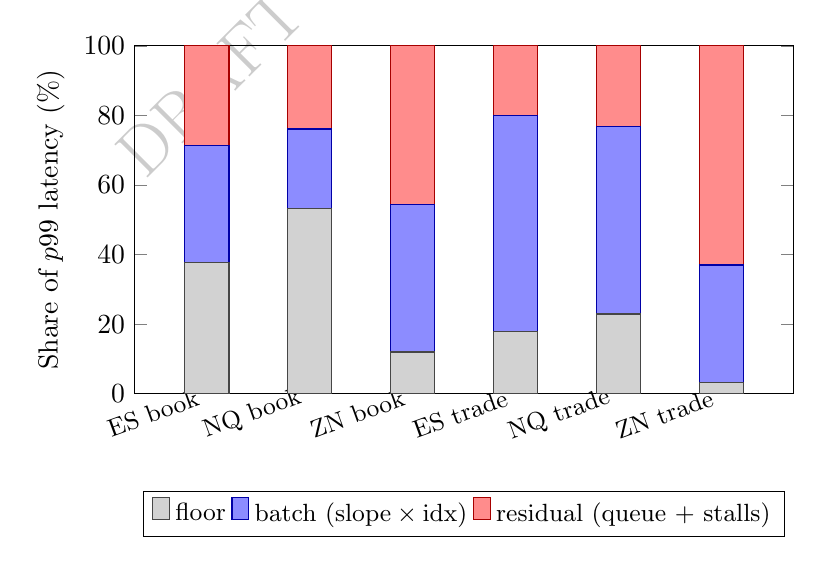
\begin{tikzpicture}
\begin{axis}[
  width=0.82\linewidth, height=6cm,
  ybar stacked, bar width=16pt,
  symbolic x coords={ES book,NQ book,ZN book,ES trade,NQ trade,ZN trade},
  xtick=data, x tick label style={rotate=20,anchor=east,font=\small},
  ymin=0, ymax=100, ylabel={Share of $p99$ latency (\%)},
  legend style={at={(0.5,-0.28)},anchor=north,legend columns=3,font=\small},
  legend cell align=left, enlarge x limits=0.14,
]
\addplot[fill=gray!35,draw=gray!55!black] coordinates {
  (ES book,37.7) (NQ book,53.2) (ZN book,12.0) (ES trade,17.9) (NQ trade,22.9) (ZN trade,3.1)};
\addplot[fill=blue!45,draw=blue!65!black] coordinates {
  (ES book,33.7) (NQ book,22.9) (ZN book,42.4) (ES trade,62.0) (NQ trade,53.9) (ZN trade,33.9)};
\addplot[fill=red!45,draw=red!65!black] coordinates {
  (ES book,28.6) (NQ book,23.9) (ZN book,45.6) (ES trade,20.1) (NQ trade,23.2) (ZN trade,63.0)};
\legend{floor, batch ($\text{slope}\times\text{idx}$), residual (queue $+$ stalls)}
\end{axis}
\end{tikzpicture}
\caption{\textbf{The tail is not the floor.} Composition of each stream's $p99$
socket-to-book latency: the floor, the in-packet batch
($\text{slope}\times\text{idx}$ evaluated at the $p99$ position), and the residual
(queue and stalls); absolute $p99$ ranges from $13.6$ to $219.4~\mu$s
(Table~\ref{tab:laddercheck}). The floor --- decode, book, and the actor framework
--- is a minority of the tail and falls to $3$--$12\%$ on the worst streams (ZN);
the structured growth is the batch term. The queue, which fires on $0.08\%$ of
messages, is only a small part of the residual; the remainder is the stall
population.}
\label{fig:tailcomp}
\end{figure}

\paragraph{Three approaches that do not help.} \emph{Reducing the message rate.}
The ranking runs the other way: NQ~book is the busiest stream ($806$ packets/s) and
has the best $p99$ ($13.6~\mu$s); ZN~book is the quietest ($241$ packets/s) and the
worst ($57.0~\mu$s). During the FOMC release ZN~book grew faster --- $12.4 \to
7.7~\mu$s --- at ten times the packet rate. A stage with $\rho$ far from $1$ does
not behave like one near saturation, and this one is not: $87\%$ to $99.7\%$ of
messages arrive to an empty ring. \emph{Sizing the ring.} Those same fractions show
most messages never queue; added ring capacity changes nothing at the median or at
the $p99$ of the book streams. The queue is real --- $\text{qlen}\ge 3$ costs
$+1.5~\mu$s at $p50$ and $+21$ to $+145~\mu$s at $p99$ --- but it fires on $0.08\%$
of messages. \emph{Batching harder.} The slope is charged per message regardless of
arrival pattern; coalescing does not reduce the work, it moves messages to higher
$\text{idx}$, the variable that lengthens tails. The trade streams are what a
batched book stream looks like: the same floor, $0.4\%$ of messages at
$\text{idx}=0$, and a $p99$ two to four times worse.

\paragraph{An open question on the slope.} The $3.1\times$ spread between NQ and ZN
is reproducible and unexplained. If it is cache residency, then making the cold
path cheaper means making it smaller --- harder than shaving instructions. If it is
message mix, ZN messages are simply more expensive and there may be nothing to win.
Resolving this requires hardware performance counters and is left open.

\FloatBarrier

\subsection{The arrival process}
\label{sec:arrival}

The sections above reduce the tail to packet span, and span is set by how many
messages arrive together --- a property of the arrival process. The natural null
is a Poisson process, and it fails in two independent ways. A Poisson process
requires both that the marginal gaps be exponentially distributed and that
successive gaps be independent; both fail here, for different reasons and with
different consequences.

\paragraph{Background: what Poisson means and how to reject it.} A \emph{Poisson
process} is the standard model of ``random, independent'' arrivals and the
assumption under which the queueing results of Section~\ref{sec:queueing} hold:
the time between successive arrivals is exponentially distributed, and each gap is
independent of the last, so arrivals neither cluster nor anticipate one another
\cite{kleinrock1975}. If the market-data feed were Poisson, packets would arrive
one at a time and evenly spread, the queue would rarely build, and the tail would
follow from utilization alone. It is not, and four standard statistics measure how
far it departs. The \emph{coefficient of variation} (CV) is the standard deviation
of the gaps over their mean; it is exactly $1$ for a Poisson process and larger
when the gaps are more uneven than exponential. The \emph{Fano factor}
\cite{fano1947} is the variance of the number of arrivals in a fixed window
divided by the mean of that count; it is $1$ for a Poisson process at every window
size, rises above $1$ when arrivals cluster, and keeps rising \emph{with the
window} when the clustering persists across timescales. The \emph{Hurst exponent}
$H$ \cite{hurst1951} summarizes that scaling: $H=0.5$ for a Poisson or any
independent process, whereas $H>0.5$ signals long-range dependence --- bursts
nested within bursts rather than one characteristic clump size. To decide whether
a departure is due to the \emph{sizes} of the gaps or their \emph{order}, we apply
a \emph{Fisher--Yates shuffle} \cite{fisheryates1938} --- the standard algorithm
that puts a list into a uniformly random order (the computing equivalent of a fair
shuffle of a deck of cards, with every one of the $n!$ orderings equally likely).
Applied to the sequence of gaps it keeps the exact multiset of gap sizes unchanged
and destroys only their order, so any statistic that falls after shuffling was
measuring order, not size.
Finally, a \emph{Hawkes process} \cite{hawkes1971,bacry2015} is a self-exciting
point process in which each arrival transiently raises the rate of further
arrivals --- a model of contagion or momentum --- whose \emph{branching ratio} is
the mean number of further arrivals each arrival directly triggers; a value near
$1$ is ``near-critical'' and produces large, long bursts. Figure~\ref{fig:raster}
gives the intuition; the rest of this section makes it quantitative.

\begin{figure}[!htb]
\centering
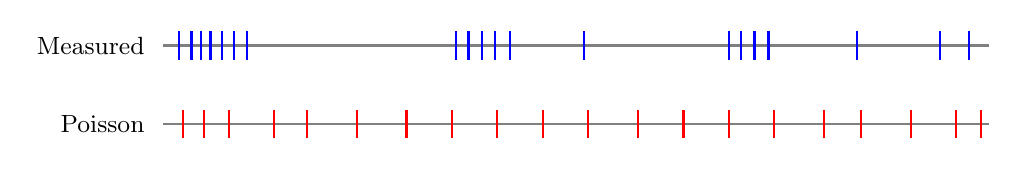
\begin{tikzpicture}[x=1.05cm]
  \node[left] at (-0.1,1.0) {\small Measured};
  \draw[thick,gray] (0,1.0) -- (10,1.0);
  \foreach \x in {0.2,0.35,0.47,0.58,0.72,0.86,1.02,3.55,3.7,3.86,4.02,4.2,5.1,6.85,7.0,7.16,7.33,8.4,9.4,9.75}
    \draw[blue,thick] (\x,0.82) -- (\x,1.18);
  \node[left] at (-0.1,0.0) {\small Poisson};
  \draw[thick,gray] (0,0.0) -- (10,0.0);
  \foreach \x in {0.25,0.5,0.8,1.35,1.75,2.35,2.95,3.5,4.05,4.6,5.15,5.75,6.3,6.85,7.4,8.0,8.45,9.05,9.6,9.9}
    \draw[red,thick] (\x,-0.18) -- (\x,0.18);
\end{tikzpicture}
\caption{\textbf{Why the feed is not Poisson (schematic).} Each row contains the
same number of packet arrivals over the same interval. A Poisson process of that
average rate spreads them out (bottom); the measured feed clusters them into
bursts separated by idle gaps (top). The clustering is what fills the ring and
enlarges packets. It is quantified --- not invented --- in
Figure~\ref{fig:fano} and Tables~\ref{tab:expgap}--\ref{tab:order}, where the
measured process reaches a Fano factor above $1000$ against Poisson's $1$. The
tick positions here are illustrative, not the measured timestamps.}
\label{fig:raster}
\end{figure}

One sampling note: the two tests below read raw packet arrival timestamps from a
separate side file (arrival times only, no latency), over the whole capture after
the startup replay rather than the $14$:$25$--$15$:$18$ latency window. The sample
$n$ is therefore larger than in the latency tables and the rates differ slightly;
the Fano statistic at a $5$-second window needs the full span.

\paragraph{The marginal is not exponential.} The fair null is an exponential with
the same mean, which fixes the average rate so that every difference is shape
rather than level; for $\text{Exp}(1/m)$ the $p$-th quantile is $-m\ln(1-p)$.
Table~\ref{tab:expgap} compares the two on ES~book. The ratio is below $1$ through
$p90$ and above $1$ in the tail, crossing once: most packets arrive far closer
together than a Poisson of the same rate would place them, paid for by rare long
idles --- the signature of a burst process.

\begin{table}[!htb]
\centering
\caption{\textbf{ESZ6 book interarrival gaps against an exponential of the same
mean} ($n=4{,}154{,}158$, mean gap $1793.6~\mu$s, rate $557.5$/s). The ratio
crosses $1$ once.}
\label{tab:expgap}
\small
\begin{tabular}{lrrr}
\toprule
Quantile & Measured ($\mu$s) & Exp, same mean ($\mu$s) & Ratio \\
\midrule
$p10$   & \phantom{000}7.22 & \phantom{0}188.97 & $0.04\times$ \\
$p50$   & \phantom{00}74.60 & 1243.22 & $0.06\times$ \\
$p90$   & \phantom{0}3196.83 & 4129.88 & $0.77\times$ \\
$p99$   & 32182.96 & 8259.77 & $3.90\times$ \\
$p99.9$ & 119057.18 & 12389.65 & $9.61\times$ \\
\bottomrule
\end{tabular}
\end{table}

The quantity that matters for a ring buffer is the share of packets that arrive
nearly on top of the one before. For any exponential this is a constant,
$P(\text{gap}<\text{mean}/10)=1-e^{-0.1}=9.52\%$. Table~\ref{tab:cvgap} shows it
reaching $85\%$ on ZN~book: these are the back-to-back runs that fill the ring and
enlarge the packet, and a Poisson source at the identical average rate would
essentially never deliver them. Both CV and CV$^2$ are tabulated with their
definitions, since the two are frequently confused.

\begin{table}[!htb]
\centering
\caption{\textbf{Interarrival-gap dispersion.} CV is the coefficient of variation
of the gaps and CV$^2$ its square. $P(\text{gap}<\text{mean}/10)$ is the share of
near-back-to-back arrivals; for any exponential it is $9.52\%$.}
\label{tab:cvgap}
\small
\begin{tabular}{lrrrr}
\toprule
Stream & CV & CV$^2$ & $P(\text{gap}<\text{mean}/10)$ & vs Poisson $9.52\%$ \\
\midrule
ES book  & 10.97 & 120.4 & $73.94\%$ & $7.8\times$ \\
NQ book  & 28.97 & 839.1 & $63.11\%$ & $6.6\times$ \\
ZN book  & 13.60 & 184.9 & $84.82\%$ & $8.9\times$ \\
ES trade &  4.10 &  16.8 & $56.01\%$ & $5.9\times$ \\
NQ trade &  4.78 &  22.8 & $39.97\%$ & $4.2\times$ \\
ZN trade &  6.11 &  37.4 & $84.20\%$ & $8.8\times$ \\
\bottomrule
\end{tabular}
\end{table}

Equivalently, the decoder never experiences the average rate.
Table~\ref{tab:rate} contrasts the mean packet rate with the instantaneous rate
implied by the median gap; for an exponential that ratio is $1/\ln 2 = 1.44\times$
at any rate. ZN~book is quoted at $241$ packets per second, yet the typical
back-to-back pair arrives at an instantaneous rate near twenty-nine thousand.

\begin{table}[!htb]
\centering
\caption{\textbf{The decoder does not experience the average rate.} Mean packet
rate against the instantaneous rate implied by the median gap. For an exponential
the ratio is $1.44\times$.}
\label{tab:rate}
\small
\begin{tabular}{lrrr}
\toprule
Stream & Mean rate & Rate from median gap & Ratio \\
\midrule
ES book & $557.5$/s & $13{,}405$/s & $24.1\times$ \\
NQ book & $806.0$/s & $11{,}555$/s & $14.3\times$ \\
ZN book & $240.9$/s & $29{,}028$/s & $120.5\times$ \\
\bottomrule
\end{tabular}
\end{table}

\paragraph{The order is not independent either.} A non-exponential marginal alone
would still admit a renewal process --- heavy-tailed gaps drawn independently.
The control is a seeded Fisher--Yates shuffle of the gap sequence, which preserves
the marginal exactly and destroys only the ordering; if the burstiness lived in
the marginal, the shuffle would change nothing. Table~\ref{tab:order} reports the
result. Gap autocorrelation is positive at all seven lags tested on all six
streams ($42$ of $42$ outside the white-noise band): long gaps follow long, short
follow short. The Fano factor --- variance of the count in a window over its mean,
$1.0$ for Poisson at every window size --- reaches $1024$--$1260$ on the book
streams at a $5$-second window and collapses by $2.8\times$ to $18.5\times$ under
the shuffle. That collapse is the result: the burstiness lives in the ordering,
because the shuffle left the marginal untouched and still removed most of it. Fano
scaling gives $\text{Fano}(T)\sim T^{2H-1}$; the measured Hurst exponent is
$0.643$--$0.743$ against a shuffled null of $0.600$--$0.660$ and $0.5$ for any
renewal process. If the generating process is Hawkes, the Fano ceiling implies a
branching ratio $n\le 1-1/\sqrt{\text{Fano}}$ of $0.850$ to $0.972$ --- each
arrival triggering close to one further arrival, a system just below criticality.

\begin{table}[!htb]
\centering
\caption{\textbf{Ordering statistics.} Gap ACF~L1 is the lag-1 gap
autocorrelation; Fano(5s) is the count Fano factor at a $5$-second window
($1.0$ for Poisson at any window); \emph{shuffled} recomputes it after a seeded
Fisher--Yates shuffle of the gap sequence, which preserves the marginal and
destroys the order; \emph{collapse} is their ratio. $H$ is the Hurst exponent from
Fano scaling ($0.5$ for Poisson or any renewal process); $H$~shuffled is the same
on the shuffled series.}
\label{tab:order}
\small
\begin{tabular}{lrrrrrr}
\toprule
Stream & gap ACF L1 & Fano(5s) & shuffled & collapse & $H$ & $H$ shuffled \\
\midrule
ES book  & $+0.040$ & 1024.2 & \phantom{0}55.3 & $18.5\times$ & 0.743 & 0.622 \\
NQ book  & $+0.005$ & 1260.0 & 103.1 & $12.2\times$ & 0.702 & 0.660 \\
ZN book  & $+0.052$ & 1133.5 & \phantom{0}69.4 & $16.3\times$ & 0.711 & 0.624 \\
ES trade & $+0.131$ & \phantom{00}65.6 & \phantom{0}12.8 & $5.1\times$ & 0.680 & 0.604 \\
NQ trade & $+0.065$ & \phantom{00}44.3 & \phantom{00}7.1 & $6.2\times$ & 0.695 & 0.600 \\
ZN trade & $+0.284$ & \phantom{00}73.0 & \phantom{0}25.7 & $2.8\times$ & 0.643 & 0.615 \\
\bottomrule
\end{tabular}
\end{table}

Two caveats. The shuffle is not a control for a slowly drifting rate, which
shuffling also destroys; this sample cannot separate self-excitation from
non-stationarity, and both read as clustering. And the shuffled null is
$0.60$--$0.66$, not $0.5$ --- finite-sample bias in the Hurst estimator at these
window counts --- so the effect is the gap between $0.74$ and $0.62$, not the
distance from $0.5$.

\begin{figure}[!htb]
\centering
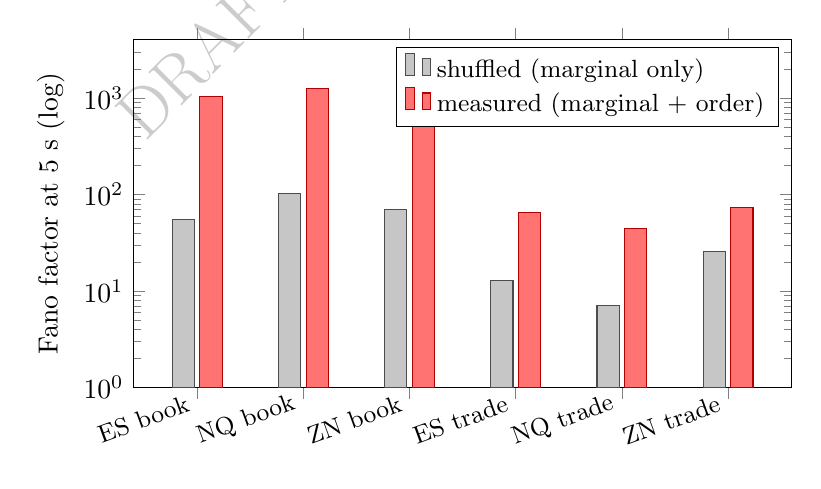
\begin{tikzpicture}
\begin{axis}[
  width=0.82\linewidth, height=6cm,
  ybar, bar width=8pt, ymode=log, log origin=infty,
  symbolic x coords={ES book,NQ book,ZN book,ES trade,NQ trade,ZN trade},
  xtick=data, x tick label style={rotate=20,anchor=east,font=\small},
  ymin=1, ymax=4000, ylabel={Fano factor at $5$~s (log)},
  legend style={at={(0.98,0.98)},anchor=north east,font=\small},
  legend cell align=left, enlarge x limits=0.12,
]
\addplot[fill=gray!45,draw=gray!60!black] coordinates {
  (ES book,55.3) (NQ book,103.1) (ZN book,69.4) (ES trade,12.8) (NQ trade,7.1) (ZN trade,25.7)};
\addplot[fill=red!55,draw=red!70!black] coordinates {
  (ES book,1024.2) (NQ book,1260.0) (ZN book,1133.5) (ES trade,65.6) (NQ trade,44.3) (ZN trade,73.0)};
\legend{shuffled (marginal only), measured (marginal $+$ order)}
\end{axis}
\end{tikzpicture}
\caption{\textbf{Two reasons the arrivals beat Poisson.} Count Fano factor at a
$5$-second window (Table~\ref{tab:order}); Poisson is $1$ at every window --- the
baseline at the bottom of the axis. The shuffled bar, with the gap sequence
reordered and the marginal preserved, is the burstiness the marginal alone
carries; the measured bar adds the ordering. Both tower over the Poisson
baseline, and the measured/shuffled gap ($2.8$--$18.5\times$) is contributed by
correlation that a marginal statistic such as $c_a^2$ cannot see.}
\label{fig:fano}
\end{figure}

\paragraph{Why this lengthens the tail beyond Poisson.} The mechanism is
mechanical. Clustered arrivals place several packets inside one decode interval;
CME coalesces what it can into a single datagram, so clustering converts into
span --- more SBE messages per UDP packet --- and span converts into latency
linearly, message $k$ paying $k\times\text{slope}$ at $0.31$--$0.97~\mu$s per
message with no randomness. A Poisson source at $557$ packets/s would leave
$1.79$~ms between packets and deliver a span-$1$ packet almost every time; the
measured stream has a $74~\mu$s median gap and span-$45$ packets, and the last
message of one pays $44\times0.57=25~\mu$s of serialization on top of a $7~\mu$s
floor. The tail originates in the arrival process: clustering becomes packet span,
and span becomes latency through the slope.

This is also why the standard queueing correction is insufficient. Kingman's
approximation \cite{kingman1961}
$\mathbb{E}[W]\approx\frac{\rho}{1-\rho}\cdot\frac{c_a^2+c_s^2}{2}\cdot\mathbb{E}[S]$
admits burstiness only through $c_a^2$, the squared CV of the marginal, and
understates here in two independent ways. First, the shuffle shows that
correlation contributes beyond anything the marginal can explain, and $c_a^2$
cannot see ordering. Second, $\rho$ is far from $1$ --- $87\%$ to $99.7\%$ of
messages find the ring empty --- so the $\rho/(1-\rho)$ term does almost no work.
The queue term is small and the variability term is blind to the mechanism that
actually produces the tail. The queue in front of the packet is convex, as
Section~\ref{sec:queue-deconf} shows, fires on $0.08\%$ of messages, and when it
fires costs $+1.5~\mu$s at the median and $+21$ to $+145~\mu$s at $p99$: a rare,
sharp effect on top of a common, smooth one. The batch accounts for the bulk of
the tail mass; the queue accounts for why the far tail exceeds what the batch
alone predicts.

\begin{figure}[!htb]
\centering
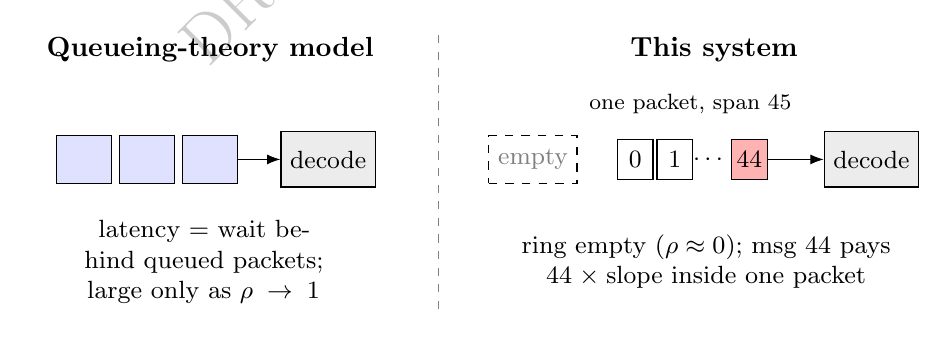
\begin{tikzpicture}[font=\small,
  pkt/.style={draw, fill=blue!12, minimum height=6mm, minimum width=7mm},
  cell/.style={draw, minimum height=5mm, minimum width=4.5mm, inner sep=1pt},
  dec/.style={draw, fill=gray!15, minimum width=10mm, minimum height=7mm},
]
\node[font=\bfseries] at (1.0,2.6) {Queueing-theory model};
\node[pkt] (p1) at (-0.6,1.2) {};
\node[pkt] (p2) at (0.2,1.2) {};
\node[pkt] (p3) at (1.0,1.2) {};
\node[dec] (d1) at (2.5,1.2) {decode};
\draw[-{Latex}] (p3.east) -- (d1.west);
\node[align=center, text width=4.2cm] at (0.9,-0.1)
  {latency $=$ wait behind queued packets; large only as $\rho \to 1$};
\draw[dashed, gray] (3.9,-0.7) -- (3.9,2.8);
\node[font=\bfseries] at (7.4,2.6) {This system};
\node[draw, dashed, minimum width=11mm, minimum height=6mm, text=gray] (ring) at (5.1,1.2) {empty};
\node[cell] (c0) at (6.4,1.2) {0};
\node[cell] (c1) at (6.9,1.2) {1};
\node at (7.35,1.2) {$\cdots$};
\node[cell, fill=red!30] (c44) at (7.85,1.2) {44};
\node[dec] (d2) at (9.4,1.2) {decode};
\node at (7.1,1.9) {\footnotesize one packet, span 45};
\draw[-{Latex}] (c44.east) -- (d2.west);
\node[align=center, text width=4.7cm] at (7.3,-0.1)
  {ring empty ($\rho \approx 0$); msg~44 pays $44 \times \text{slope}$ inside one packet};
\end{tikzpicture}
\caption{\textbf{Why queueing theory misses the tail.} The M/M/1 model charges
latency to packets waiting in the mailbox, which is large only near saturation.
In the measured system the ring is empty $87$--$99.7\%$ of the time
($\rho \approx 0$), yet one coalesced packet can carry dozens of messages, and
the $k$-th pays $k \times \text{slope}$ of serialization before it is decoded ---
a tail the queueing model cannot see, because it assumes one service per arrival.}
\label{fig:whyqueue}
\end{figure}

\subsection{Limits of this measurement}

$t_0$ is a software timestamp at the socket read, so this is socket-to-book, not
wire-to-book; hardware receive timestamps would close that gap and were not taken.
The data is one box and one $53$-minute session; a $12$-minute cut of the same
session gave per-message slopes that moved by up to $2.4\times$, so this window is
not obviously sufficient either. The per-message service cost varies $\sim\!3\times$
across instruments (ZN is dearest), and whether that is cold-cache residency or a
genuinely heavier message mix cannot be separated without hardware counters. The
deep-queue rows ($\text{qlen}\ge5$) are too sparse to characterize their tail, so
the queue result rests on queue lengths $0$--$3$ on the three book streams. And a
separate population of multi-millisecond stalls --- the largest latencies in the
dataset --- is real and remains unexplained here.

% ---------------------------------------------------------------
\section{Production and simulation: a duality of the group}
\label{sec:duality}
% ---------------------------------------------------------------

\paragraph{The group defines a single message order.} A \texttt{Group}
co-schedules its member actors on one thread behind one shared mailbox
(Section~\ref{sec:micro}): the members do not own separate queues; the group's
single queue holds every message addressed to any member, and the run loop
dispatches them one at a time. Beyond the latency effect measured earlier --- the
collapse of the round trip from $\sim\!3.4\,\mu$s to $90$~ns --- this has a
structural consequence. A single queue imposes a single total order on all
messages entering the group, so the group's entire execution --- every actor
state transition and every outgoing message --- is a deterministic function of
that one input sequence.

\paragraph{The same actors run in production and in simulation.} That property
makes one group two systems. In production the queue is fed by live sources ---
socket readers, timers, market-data actors --- and the run loop executes in real
time. In simulation the queue is fed from a recorded or synthetic sequence, and
the run loop executes as fast as the host permits. The member actors are
identical in both modes: a handler cannot determine whether the message it is
processing arrived from a live socket or a backtest file, which is the receiver
transparency of Section~\ref{sec:transparency} extended from the delivery
mechanism to the data source. No strategy actor is edited, recompiled, or
conditionally branched to move between live trading and backtest, and replaying
the same input sequence reproduces the same states and outputs. The one
discipline the duality imposes on an actor is that it acquire time, randomness,
and external input through messages or injected interfaces rather than through
global calls, so that the simulator can supply them deterministically.

\paragraph{Relation to prior work.} Two ingredients of this design have prior
art; their combination is uncommon. The single-shared-queue group is a
first-class facility in Actor4j \cite{actor4j2018}, where a group's actors run on
one thread with their mailboxes outsourced to the thread's queue --- presented
there as a message-passing throughput optimization, not as a simulation
mechanism. The same-code production/simulation duality is the principle of
deterministic simulation testing: FoundationDB's Flow runtime \cite{foundationdb}
and systems such as TigerBeetle run unmodified production code inside a
single-threaded deterministic simulator, but there the unit of determinism is an
asynchronous continuation or an explicit state machine rather than a group of
mailbox actors sharing a queue. Agent-based market simulators such as ABIDES
\cite{abides} drive actor-like agents behind one time-ordered event queue, but
those agents exist only in simulation and are not a deployed production system.
The design here couples the two: the shared-queue group is the seam that makes
mode-agnostic actors run identically in real-time production and in deterministic
backtest. We are not aware of this specific combination being described
elsewhere.

\paragraph{Example: developing an execution algorithm.} This duality is how the
order-level shadowing execution algorithm of the companion paper \cite{shadowpov}
was developed. The strategy is an actor that consumes market-data and order-event
messages and emits child-order messages; it was built and validated entirely in
simulation, driven from recorded CME sessions, and then deployed to production
without modification --- the same actor and the same handlers, reading from a
live feed instead of a file. The $246$-session slippage comparison reported there
was produced by the simulation mode of the same group that runs the strategy
live. The child-order logic is written once and is agnostic to the mode in which
it executes.

% ---------------------------------------------------------------
\section{Discussion and limitations}
\label{sec:disc}
% ---------------------------------------------------------------

\paragraph{The scope is co-located actors.} \fs{} applies only when sender and
receiver share an address space; a synchronous cross-machine call would
reintroduce the network round trip it exists to avoid, and the actor model's
location transparency means the sender can fall back to asynchronous delivery
when the receiver is remote. Receiver transparency is what makes that fallback
free: the same handler serves the remote asynchronous case and the local
synchronous case.

\paragraph{The cost of transparency.} Heap-allocating the reply in both modes is
a deliberate cost paid to keep the handler unable to distinguish them. The
optimized synchronous-only reply removes that allocation but forfeits
transparency and must therefore be confined to code paths statically known to be
synchronous; mixing it with asynchronous delivery is an error the mechanism
reports rather than tolerates.

\paragraph{Blocking runs counter to conventional guidance.} Established actor
frameworks discourage blocking inside actors precisely because it can starve
thread pools and cause deadlock \cite{akka,armstrong2003,swift2021}. \fs{}
blocks the sender by construction, and its safety rests on the cyclic-invocation
detector and on the availability of the non-blocking and best-effort variants for
paths that cannot tolerate an unbounded wait. Where a caller must never block,
\texttt{fast\_send\_x} and \texttt{fast\_send\_void} provide bounded-time and
never-blocking alternatives behind the same handler interface. Even so, the
cyclic-invocation detector addresses only \emph{cyclic} waits; avoiding
thread-pool starvation for acyclic blocking patterns --- a chain that blocks on
an actor whose handler is itself waiting on a scarce resource --- remains a
burden on the developer that asynchronous delivery does not impose.

\paragraph{Contention on a hot actor.} A synchronous send holds the receiver's
exclusive-access lock for the duration of handler execution, so concurrent
synchronous sends to the same heavily contended actor serialize on that lock, and
the blocking variants stall their caller threads while they wait. Under heavy
contention this can perform worse than asynchronous delivery, in which senders
enqueue and continue and the messages buffer without stalling the callers. The
non-blocking (\texttt{fast\_send\_x}) and best-effort (\texttt{fast\_send\_void})
variants bound or remove the stall --- the latter by falling back to the mailbox
--- so the ratio of synchronous completions to asynchronous fallbacks, a metric
the mechanism already exposes, doubles as a signal that a target has become hot
enough that the asynchronous path is preferable.

\paragraph{Permissive detection shifts a burden to the programmer.} The
(actor, message-class) refinement admits callbacks by allowing an actor's state
to be re-entered by a nested handler, which reintroduces the reentrancy hazards
that strict per-actor sequential processing removes. A nested handler can
observe and mutate the actor's state mid-update, which relaxes the actor model's
guarantee of single-threaded sequential state mutation and admits the invariant
violations that guarantee is designed to prevent. The conservative policy avoids
this at the cost of rejecting some legitimate callback structures; the choice
between them is exposed as configuration rather than fixed.

\paragraph{Further evaluation.} The microbenchmarks of Section~\ref{sec:micro}
establish the per-operation latency reductions and the two-order-of-magnitude
tail benefit of the memory pool directly. The natural next step measures the
mechanism under load: synchronous versus asynchronous \emph{throughput} across
contention levels, chain depths, and message sizes on the x86-64 Linux target,
together with the distribution of synchronous completions versus asynchronous
fallbacks for \texttt{fast\_send\_void}. That saturated, multi-axis
characterization is the subject of ongoing work.

% ---------------------------------------------------------------
\section{Conclusion}
% ---------------------------------------------------------------

The actor model has long been dismissed for high-frequency trading on a plausible
but mistaken premise: that its safety is inseparable from a discipline --- one
thread per actor, a mailbox per actor, a message and a context switch for every
interaction --- whose per-message cost cannot fit a microsecond budget. The
premise conflates the model with one way of implementing it. For \emph{co-located}
actors the discipline can be honored without that cost, and the resulting system
is fast enough for the HFT hot path while keeping the properties that made the
model attractive in the first place: per-actor state isolation, freedom from data
races and deadlocks, and sequential single-message reasoning. This paper supports
that thesis both analytically and with a deployed, measured implementation ---
kaspar-hft --- rather than as theory alone.

Asynchronous message passing is intrinsic to the actor model's guarantees and
indispensable across machines, but for co-located actors it imposes heap
allocation, queue operations, scheduling, and context switches that isolation
does not require. \fs{} provides a synchronous alternative in which the sender's
thread runs the receiver's handler directly under the receiver's exclusive-access
lock and takes the reply as a value, while the handler remains unable to
determine the delivery mode, the executing thread, or the sender's blocked state
--- receiver transparency. A thread-local call-chain membership test, checked
before lock acquisition, makes the cross-thread synchronous path safe against the
deadlock and stack-overflow modes that cyclic synchronous invocation would
otherwise cause, and a refinement keyed on (actor, message-class) pairs admits
legitimate callbacks while still catching unbounded recursion. Five delivery
operations expose the latency/robustness spectrum behind one transparent handler
interface. The performance case is made analytically, as the elimination of
per-message work, and corroborated by microbenchmarks in which the synchronous
path completes a round trip in tens of nanoseconds and a memory pool cuts the
latency tail by two orders of magnitude.

The applied study places these numbers against a live market-data path. On the
kaspar-hft framework, socket-to-book latency decomposes into a $\sim\!7~\mu$s
decode-and-book floor and a per-message serialization slope; the floor is stable
to within a few tenths of a microsecond across three estimators and a tenfold
change in packet rate, and the framework's own $\sim\!30$~ns hop is under $1\%$ of
it. The tail is not the framework and not, primarily, the queue: with in-packet
position held fixed the mailbox queue is convex exactly as queueing theory
predicts but fires on only $0.08\%$ of messages, while the dominant effect is the
arrival process, which is non-Poisson and self-exciting (Hawkes-like, branching
ratio $0.85$--$0.97$) and converts bursts into large packets and in-packet
position into latency through the slope. The design lever is therefore the
per-message service time, not the queue depth or the message rate. The same study
also fixes the choice among the four mailbox queue implementations --- BQueue by
default, ShardedBQueue for high-fan-in actors --- and shows that a group of actors
sharing one queue is at once a real-time execution engine and a deterministic
simulator, so a trading strategy is developed in backtest and deployed to
production without modification.

Taken together, the mechanism and the measurement answer the question in the
title. The four extensions --- \fs{}, actor groups, per-actor mailbox selection,
and the memory pool --- reduce the actor framework's contribution on a live
tick-to-book path to under one percent of the irreducible decode-and-book floor,
and to nothing in the tail, which belongs to the market's arrival process and not
to the messaging layer. An HFT data path built on this model therefore pays
essentially no latency penalty for the actor discipline, and in return obtains
data-race and deadlock freedom, single-message reasoning that is unusually
amenable to automatic code generation, and a production/simulation duality in
which the same strategy code is backtested and traded without change. The actor
model, long held unsuitable for high-frequency trading, is suitable, and a real
system trades on it. The remaining work is the saturated-throughput and
contention evaluation that this sequential study does not attempt.

% ---------------------------------------------------------------
\begin{thebibliography}{99}
% ---------------------------------------------------------------
\bibitem{hewitt1973} C.~Hewitt, P.~Bishop, and R.~Steiger.
  \emph{A Universal Modular ACTOR Formalism for Artificial Intelligence.}
  Proc.\ 3rd International Joint Conference on Artificial Intelligence (IJCAI),
  1973.
\bibitem{agha1986} G.~Agha.
  \emph{Actors: A Model of Concurrent Computation in Distributed Systems.}
  MIT Press, 1986.
\bibitem{miller2005} M.~S.~Miller, E.~D.~Tribble, and J.~Shapiro.
  \emph{Concurrency Among Strangers: Programming in E as Plan Coordination.}
  Symposium on Trustworthy Global Computing, 2005.
\bibitem{ambienttalk2007} T.~Van Cutsem et al.
  \emph{AmbientTalk: Object-Oriented Event-Driven Programming in Mobile Ad Hoc
  Networks.} XXVI Int.\ Conf.\ of the Chilean Computer Science Society, 2007.
\bibitem{armstrong1996} J.~Armstrong, R.~Virding, C.~Wikstr\"om, and M.~Williams.
  \emph{Concurrent Programming in Erlang.} Prentice Hall, 2nd ed., 1996.
\bibitem{armstrong2003} J.~Armstrong.
  \emph{Making Reliable Distributed Systems in the Presence of Software Errors.}
  PhD thesis, Royal Institute of Technology (KTH), Stockholm, 2003.
\bibitem{akka} Lightbend, Inc.
  \emph{Akka Documentation.} \url{https://akka.io/docs/}.
\bibitem{caf2014} D.~Charousset, T.~C.~Schmidt, R.~Hiesgen, and M.~W\"ahlisch.
  \emph{CAF --- The C++ Actor Framework for Scalable and Resource-Efficient
  Applications.} Proc.\ 4th Int.\ Workshop on Programming based on Actors,
  Agents, and Decentralized Control (AGERE!), 2014.
\bibitem{orleans} S.~Bykov et al.
  \emph{Orleans: Cloud Computing for Everyone.}
  Proc.\ 2nd ACM Symposium on Cloud Computing (SoCC), 2011.
\bibitem{swift2021} Apple, Inc.
  \emph{Swift Evolution Proposal SE-0306: Actors.} 2021.
\bibitem{actor4j2018} D.~Bauer.
  \emph{Actor4j: A Software Framework for the Actor Model Focusing on the
  Optimization of Message Passing.} 2018.
\bibitem{kar2021} O.~Tardieu et al.
  \emph{Reliable Actors with Retry Orchestration.} IBM Research, 2021.
\bibitem{activeobject1996} R.~G.~Lavender and D.~C.~Schmidt.
  \emph{Active Object: An Object Behavioral Pattern for Concurrent Programming.}
  Pattern Languages of Program Design 2, Addison-Wesley, 1996.
\bibitem{posa2} D.~C.~Schmidt, M.~Stal, H.~Rohnert, and F.~Buschmann.
  \emph{Pattern-Oriented Software Architecture, Volume 2: Patterns for
  Concurrent and Networked Objects.} Wiley, 2000.
\bibitem{sutter2005} H.~Sutter and J.~Larus.
  \emph{Software and the Concurrency Revolution.} ACM Queue, 3(7):54--62, 2005.
\bibitem{linguafranca2023} M.~Lohstroh, C.~Menard, S.~Bateni, and E.~A.~Lee.
  \emph{High-Performance Deterministic Concurrency using Lingua Franca.}
  arXiv:2301.02444, 2023.
\bibitem{batching2026} V.~Maciejewski.
  \emph{How Message Batching More Than Doubles Actor-Model Throughput.}
  \url{https://vincentmayeski.substack.com/p/how-message-batching-more-than-doubles}, 2026.
\bibitem{greif1975} I.~G.~Greif.
  \emph{Semantics of Communicating Parallel Processes.}
  PhD thesis, MIT, 1975. Project MAC Technical Report MAC-TR-154.
\bibitem{hewittbaker1977} C.~Hewitt and H.~Baker.
  \emph{Laws for Communicating Parallel Processes.}
  In \emph{Information Processing 77} (Proc.\ IFIP Congress 77), North-Holland,
  1977, pp.~987--992.
\bibitem{clinger1981} W.~D.~Clinger.
  \emph{Foundations of Actor Semantics.}
  PhD thesis, MIT, 1981. MIT AI Lab Technical Report AI-TR-633.
\bibitem{armstrong2007} J.~Armstrong.
  \emph{A History of Erlang.}
  Proc.\ 3rd ACM SIGPLAN Conference on the History of Programming Languages
  (HOPL III), 2007. \url{https://doi.org/10.1145/1238844.1238850}.
\bibitem{hewitt2010} C.~Hewitt.
  \emph{Actor Model of Computation: Scalable Robust Information Systems.}
  arXiv:1008.1459, 2010 (rev.\ 2015). \url{https://arxiv.org/abs/1008.1459}.
\bibitem{beambook} E.~Stenman.
  \emph{The Erlang Runtime System (The BEAM Book), chapter ``Scheduling''.}
  \url{https://github.com/happi/theBeamBook}, accessed 2026.
\bibitem{letitcrash} Lightbend (Akka Team).
  \emph{50 Million Messages per Second --- on a Single Machine.}
  \url{https://letitcrash.com/post/20397701710/50-million-messages-per-second-on-a-single},
  2012.
\bibitem{orleansmsr2014} S.~Bykov, A.~Geller, G.~Kliot, J.~R.~Larus, R.~Pandya,
  and J.~Thelin.
  \emph{Orleans: Distributed Virtual Actors for Programmability and
  Scalability.} Microsoft Research Technical Report MSR-TR-2014-41, 2014.
\bibitem{ponyorca2017} S.~Clebsch, J.~Franco, S.~Drossopoulou, A.~M.~Yang,
  T.~Wrigstad, and J.~Vitek.
  \emph{Orca: GC and Type System Co-design for Actor Languages.}
  Proc.\ ACM Program.\ Lang.\ 1(OOPSLA), Article~72, 2017.
\bibitem{camilleri2023} C.~Camilleri, J.~G.~Vella, and V.~Nezval.
  \emph{Actor Model Frameworks: An Empirical Performance Analysis.}
  In \emph{Advances in Information and Communication} (FICC 2023), Lecture Notes
  in Networks and Systems, vol.~652, Springer, 2023.
  \url{https://doi.org/10.1007/978-3-031-31153-6_37}.
\bibitem{imam2014savina} S.~M.~Imam and V.~Sarkar.
  \emph{Savina --- An Actor Benchmark Suite: Enabling Empirical Evaluation of
  Actor Libraries.} Proc.\ 4th Int.\ Workshop on Programming based on Actors,
  Agents, and Decentralized Control (AGERE!), 2014.
  \url{https://doi.org/10.1145/2687357.2687368}.
\bibitem{blessing2019} S.~Blessing, K.~Fernandez-Reyes, A.~M.~Yang,
  S.~Drossopoulou, and T.~Wrigstad.
  \emph{Run, Actor, Run: Towards Cross-Actor Language Benchmarking.}
  Proc.\ 9th Int.\ Workshop on Programming based on Actors, Agents, and
  Decentralized Control (AGERE!), 2019.
\bibitem{charousset2013} D.~Charousset, T.~C.~Schmidt, R.~Hiesgen, and
  M.~W\"ahlisch.
  \emph{Native Actors --- A Scalable Software Platform for Distributed,
  Heterogeneous Environments.} arXiv:1301.0748, 2013.
\bibitem{actix} Actix Project.
  \emph{Actix: Actor Framework for Rust --- Documentation.}
  \url{https://docs.rs/actix/}, accessed 2026.
\bibitem{tasharofi2013} S.~Tasharofi, P.~Dinges, and R.~E.~Johnson.
  \emph{Why Do Scala Developers Mix the Actor Model with Other Concurrency
  Models?} Proc.\ 27th European Conference on Object-Oriented Programming
  (ECOOP), LNCS 7920, Springer, 2013, pp.~302--326.
\bibitem{bagherzadeh2020} M.~Bagherzadeh, N.~Fireman, A.~Shawesh, and
  R.~Khatchadourian.
  \emph{Actor Concurrency Bugs: A Comprehensive Study on Symptoms, Root Causes,
  API Usages, and Differences.} Proc.\ ACM Program.\ Lang.\ 4(OOPSLA),
  Article~214, 2020. \url{https://doi.org/10.1145/3428282}.
\bibitem{torreslopez2018} C.~Torres Lopez, S.~Marr, H.~M\"ossenb\"ock, and
  E.~Gonzalez Boix.
  \emph{A Study of Concurrency Bugs and Advanced Development Support for
  Actor-based Programs.} In \emph{Programming with Actors}, LNCS 10789,
  Springer, 2018, pp.~155--185. Also arXiv:1706.07372.
\bibitem{concur2026} J.~Huang, T.~Mahmud, C.~P{\u a}s{\u a}reanu, and G.~Yang.
  \emph{CONCUR: Benchmarking LLMs for Concurrent Code Generation.}
  arXiv:2603.03683, 2026.
\bibitem{kleinrock1975} L.~Kleinrock.
  \emph{Queueing Systems, Volume 1: Theory.} Wiley-Interscience, 1975.
\bibitem{li2007} C.~Li, C.~Ding, and K.~Shen.
  \emph{Quantifying the Cost of Context Switch.} Proc.\ Workshop on Experimental
  Computer Science (ExpCS), ACM, 2007.
\bibitem{mcvoy1996} L.~McVoy and C.~Staelin.
  \emph{lmbench: Portable Tools for Performance Analysis.}
  Proc.\ USENIX Annual Technical Conference, 1996.
\bibitem{bendersky2018} E.~Bendersky.
  \emph{Measuring Context Switching and Memory Overheads for Linux Threads.}
  \url{https://eli.thegreenplace.net/2018/measuring-context-switching-and-memory-overheads-for-linux-threads/},
  2018.
\bibitem{kasparperf} V.~Maciejewski.
  \emph{kaspar-hft actor framework: C++ message-passing microbenchmarks
  (\texttt{actors/cpp/perf}).}
  \url{https://github.com/vincent212/kaspar-hft}, 2026.
\bibitem{mdlatency2026} V.~Maciejewski.
  \emph{The Queue Is Inside the Packet: Market-Data Latency Measured One Message
  at a Time.} kaspar-hft technical report
  (\texttt{tech\_reports/md\_latency\_article.md}), 2026.
  \url{https://github.com/vincent212/kaspar-hft}.
\bibitem{fixsbe} FIX Trading Community.
  \emph{Simple Binary Encoding (SBE), Version 1.0.} Technical Standard, 2020.
  \url{https://www.fixtrading.org/standards/sbe/}.
\bibitem{shadowpov} V.~Maciejewski.
  \emph{Model-Free Passive Execution via Order-Level Shadowing.} kaspar-hft
  technical report (\texttt{tech\_reports/shadow\_pov}), 2026.
  \url{https://github.com/vincent212/kaspar-hft}.
\bibitem{foundationdb} J.~Zhou, M.~Xu, A.~Shraer, et al.
  \emph{FoundationDB: A Distributed Unbundled Transactional Key Value Store.}
  In Proc.\ ACM SIGMOD, 2021. \url{https://doi.org/10.1145/3448016.3457559}.
\bibitem{abides} D.~Byrd, M.~Hybinette, and T.~H.~Balch.
  \emph{ABIDES: Towards High-Fidelity Multi-Agent Market Simulation.}
  In Proc.\ ACM SIGSIM-PADS, 2020. \url{https://doi.org/10.1145/3384441.3395986}.
\bibitem{kingman1961} J.~F.~C.~Kingman.
  \emph{The Single Server Queue in Heavy Traffic.}
  Mathematical Proceedings of the Cambridge Philosophical Society,
  57(4):902--904, 1961. \url{https://doi.org/10.1017/S0305004100036094}.
\bibitem{fano1947} U.~Fano.
  \emph{Ionization Yield of Radiations. II. The Fluctuations of the Number of
  Ions.} Physical Review, 72(1):26--29, 1947.
  \url{https://doi.org/10.1103/PhysRev.72.26}.
\bibitem{hurst1951} H.~E.~Hurst.
  \emph{Long-Term Storage Capacity of Reservoirs.} Transactions of the American
  Society of Civil Engineers, 116:770--799, 1951.
  \url{https://doi.org/10.1061/TACEAT.0006518}.
\bibitem{hawkes1971} A.~G.~Hawkes.
  \emph{Spectra of Some Self-Exciting and Mutually Exciting Point Processes.}
  Biometrika, 58(1):83--90, 1971. \url{https://doi.org/10.1093/biomet/58.1.83}.
\bibitem{bacry2015} E.~Bacry, I.~Mastromatteo, and J.-F.~Muzy.
  \emph{Hawkes Processes in Finance.} Market Microstructure and Liquidity,
  1(1):1550005, 2015. \url{https://doi.org/10.1142/S2382626615500057}.
\bibitem{fisheryates1938} R.~A.~Fisher and F.~Yates.
  \emph{Statistical Tables for Biological, Agricultural and Medical Research.}
  Oliver \& Boyd, London, 1938. (Shuffle algorithm; see also D.~E.~Knuth,
  \emph{The Art of Computer Programming}, Vol.~2, Algorithm~P.)
\end{thebibliography}

\end{document}
